\section{Experiments and Results}

\subsection{Robot Planner 1}

In this first experiment we are testing some simple trajectories with the surgical tool already attached to the robot arm's end effector.
The path is designed using the appropriate coordinates and orientations so that the robot begins from the home position, then visits the table with the surgical 
tools and then visits the other table on top of which the mounting dock is placed. Upon arrival at the mounting dock, the robot inserts the tool inside a hole
(we consider these holes to be a simplistic alternative to the trocars used in real operations), then executes a simple pivot motion, while the tool is still 
inserted and then the tool gets ejected from the mounting dock's hole.\\

The aim of this experiment is to test the overall behaviour of the robot inside the work space, before implementing more complex path planning algorithms.

\begin{center}
\begin{figure}[H]
\centering
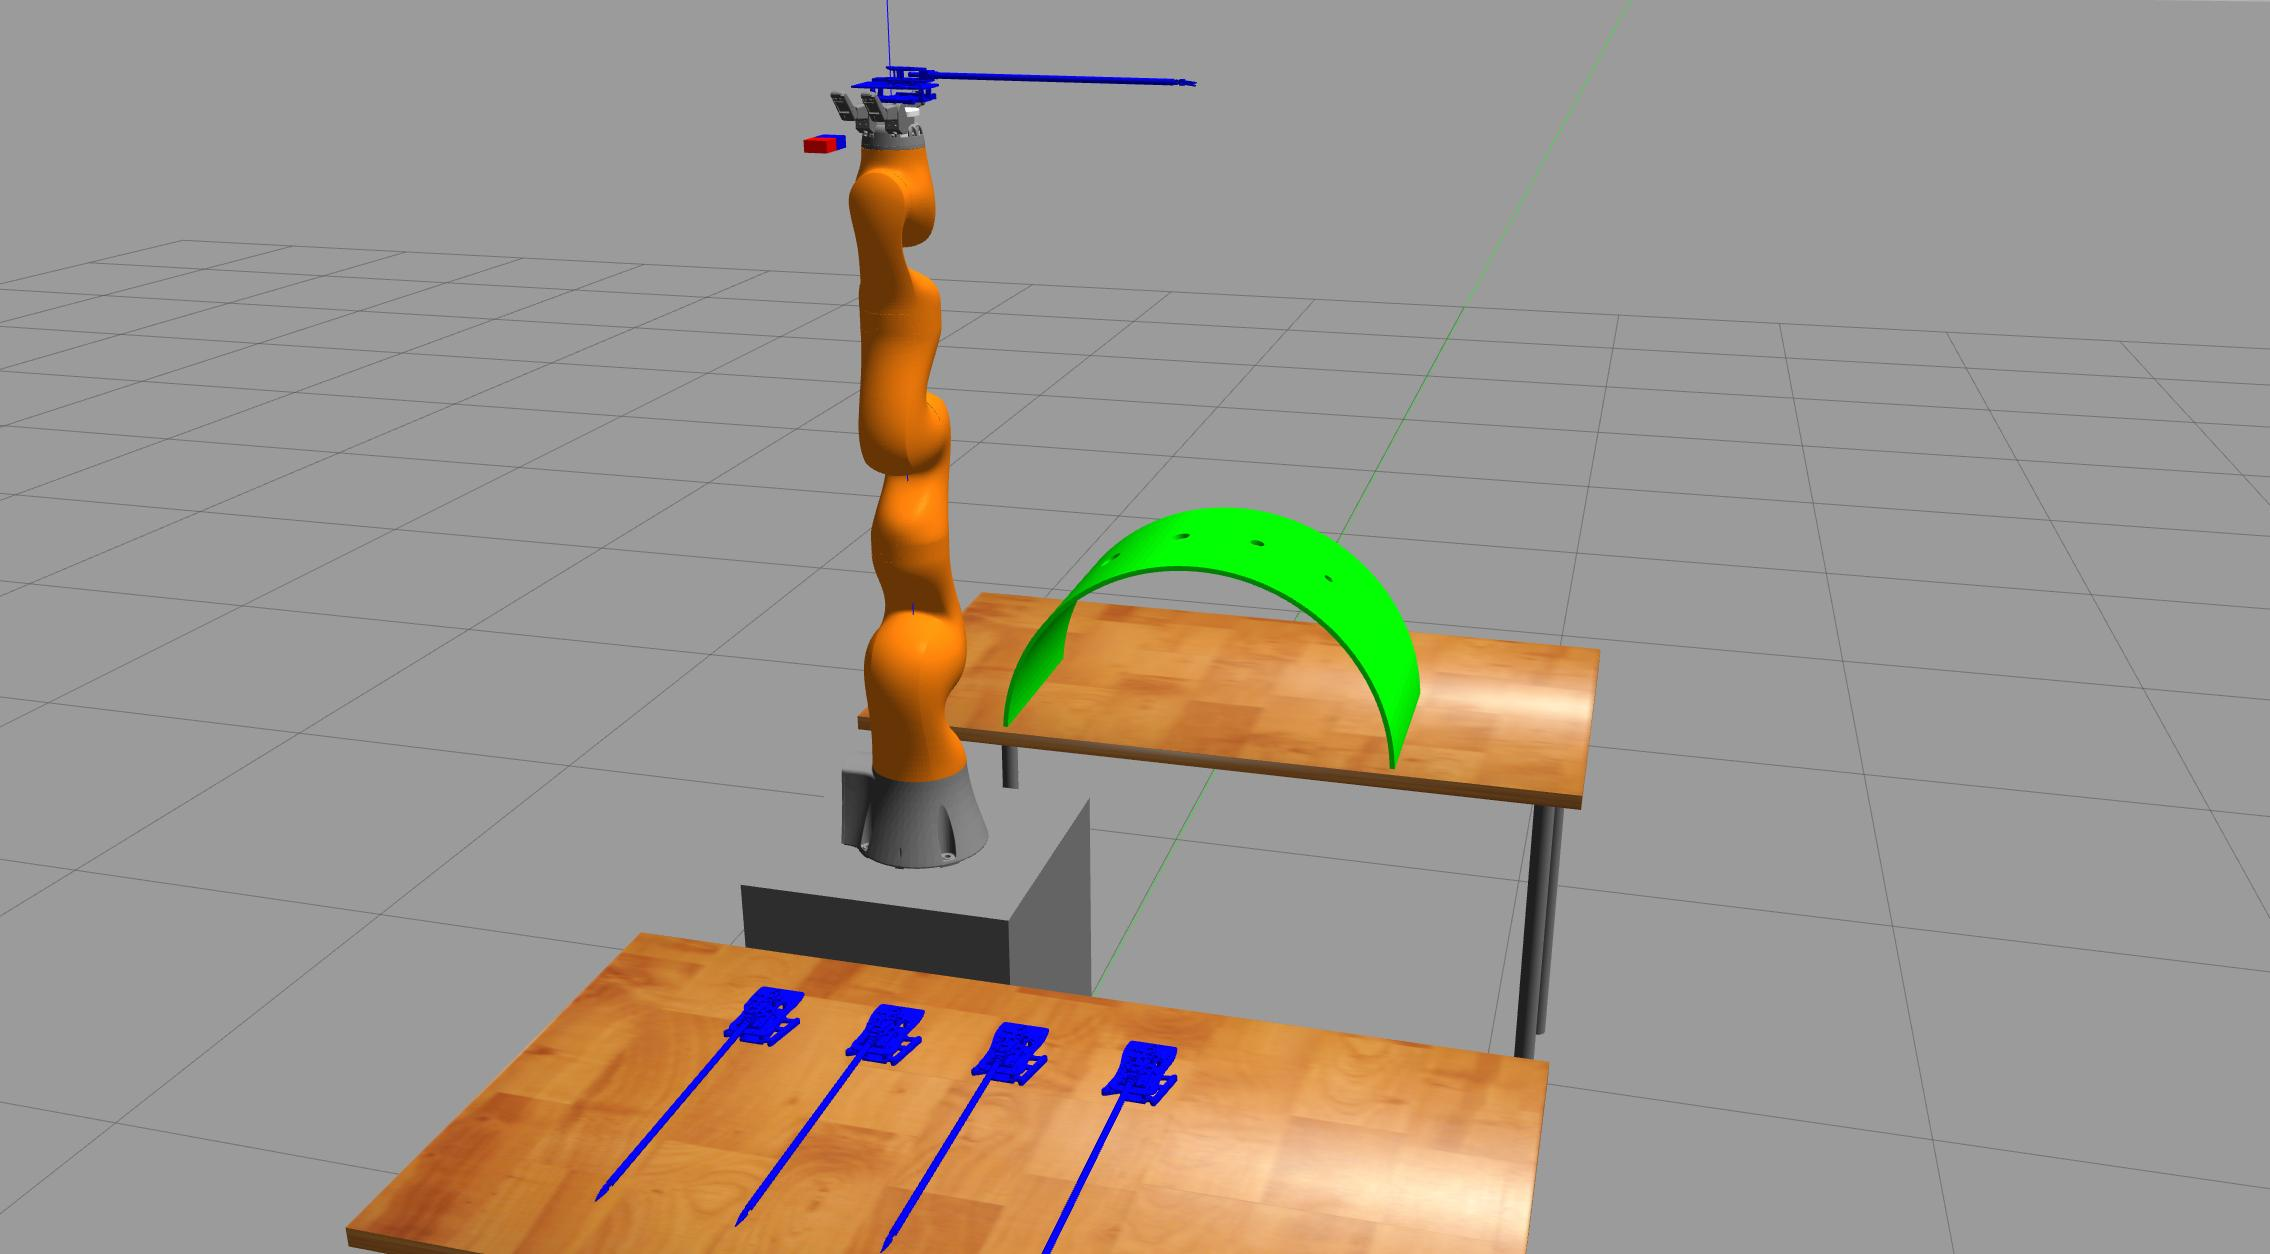
\includegraphics[width=0.3\textwidth]{images/robot_planner1/robot_planner1_1}
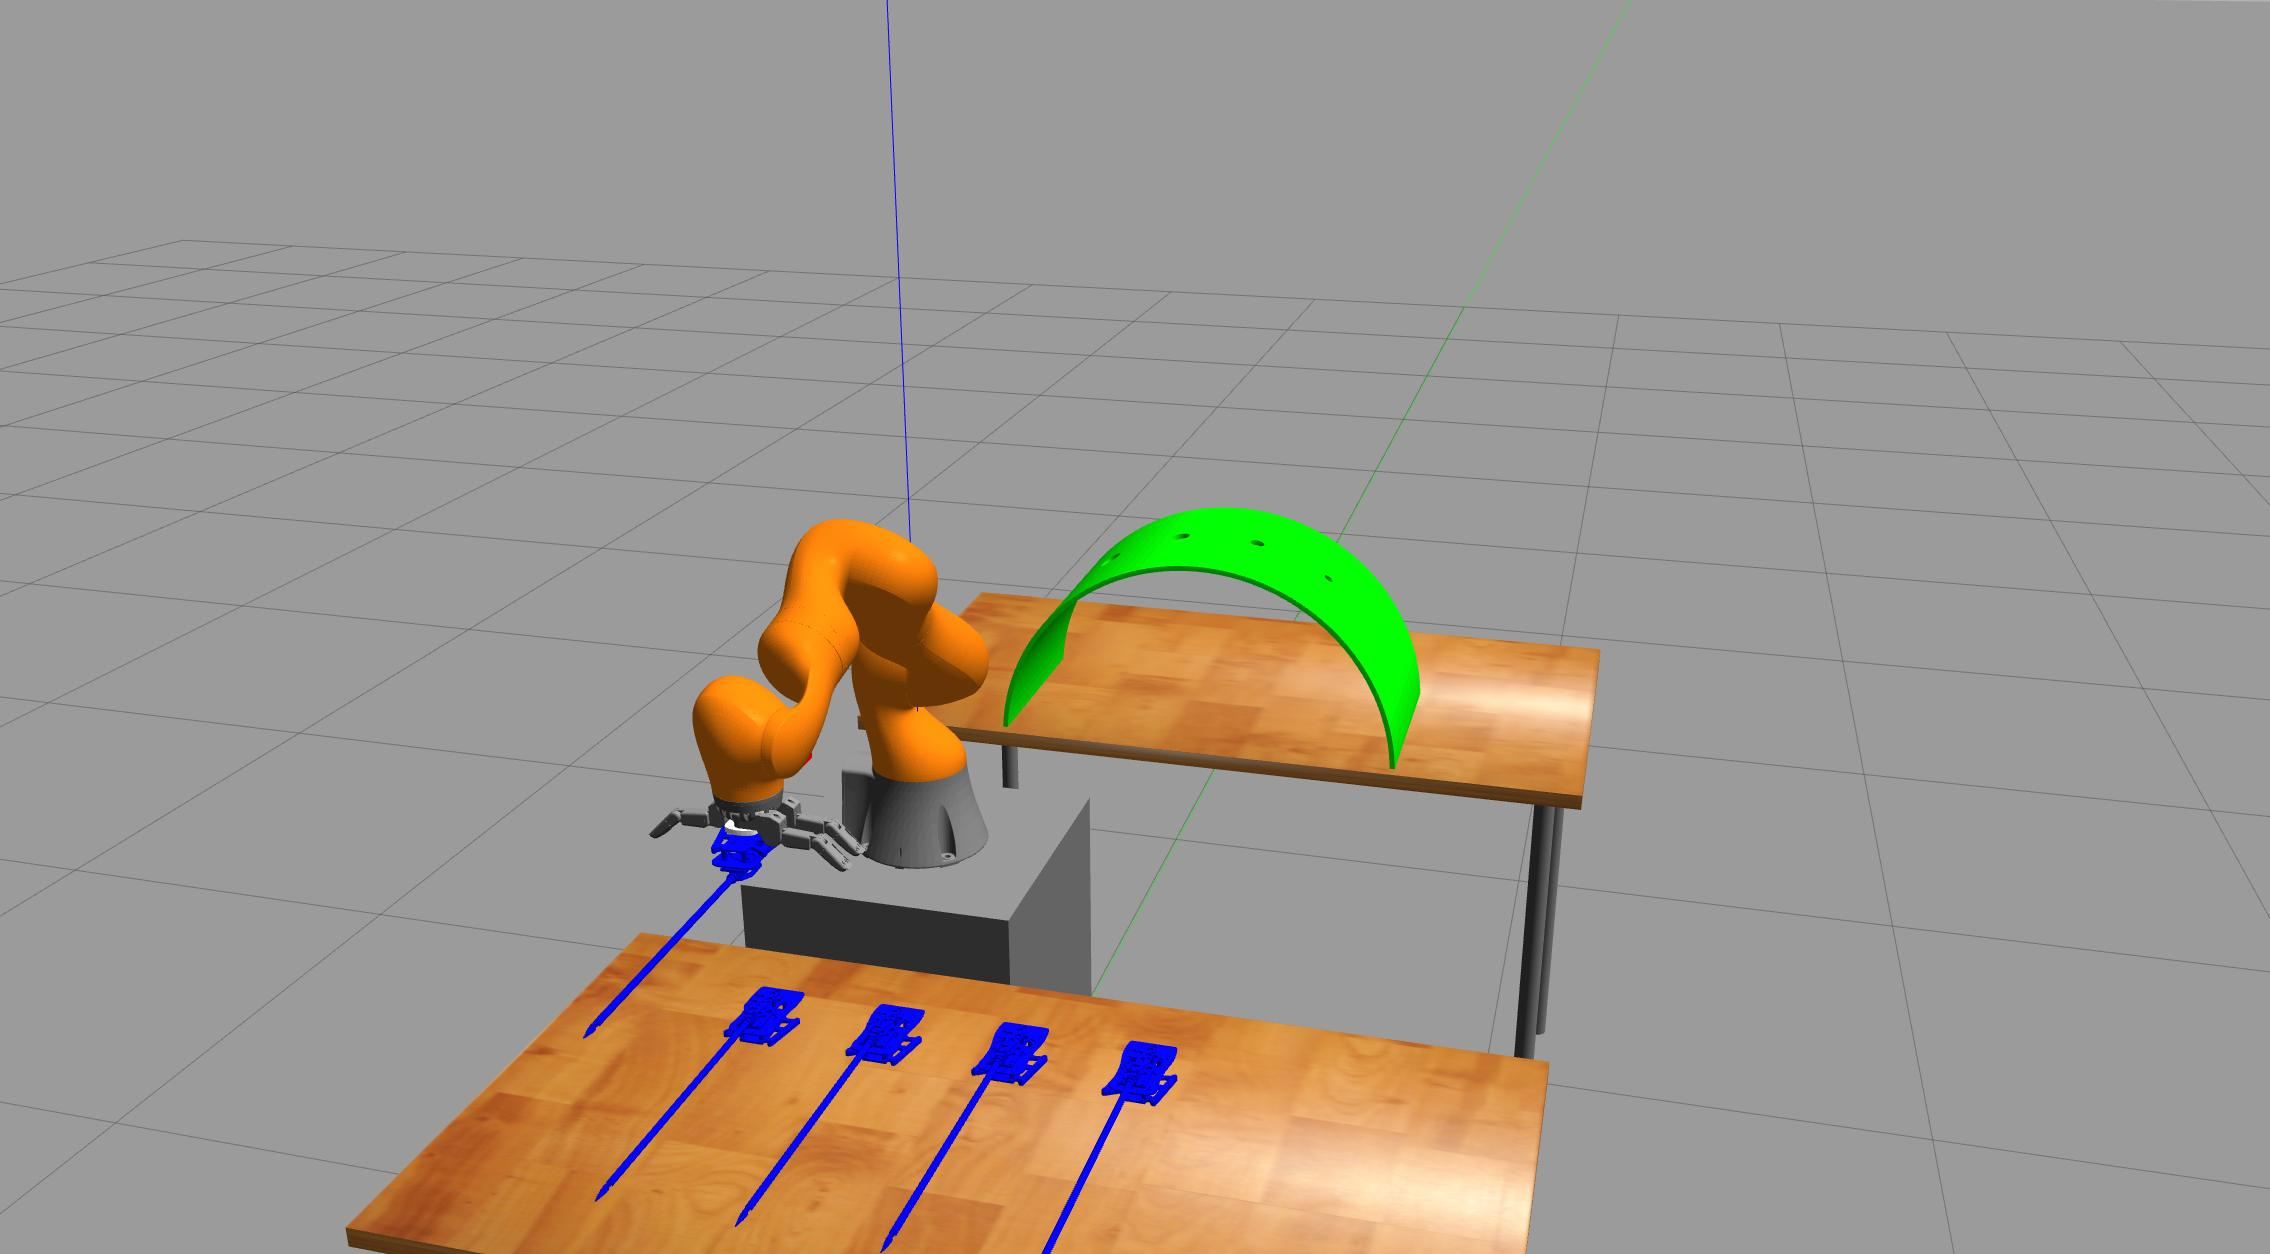
\includegraphics[width=0.3\textwidth]{images/robot_planner1/robot_planner1_2}
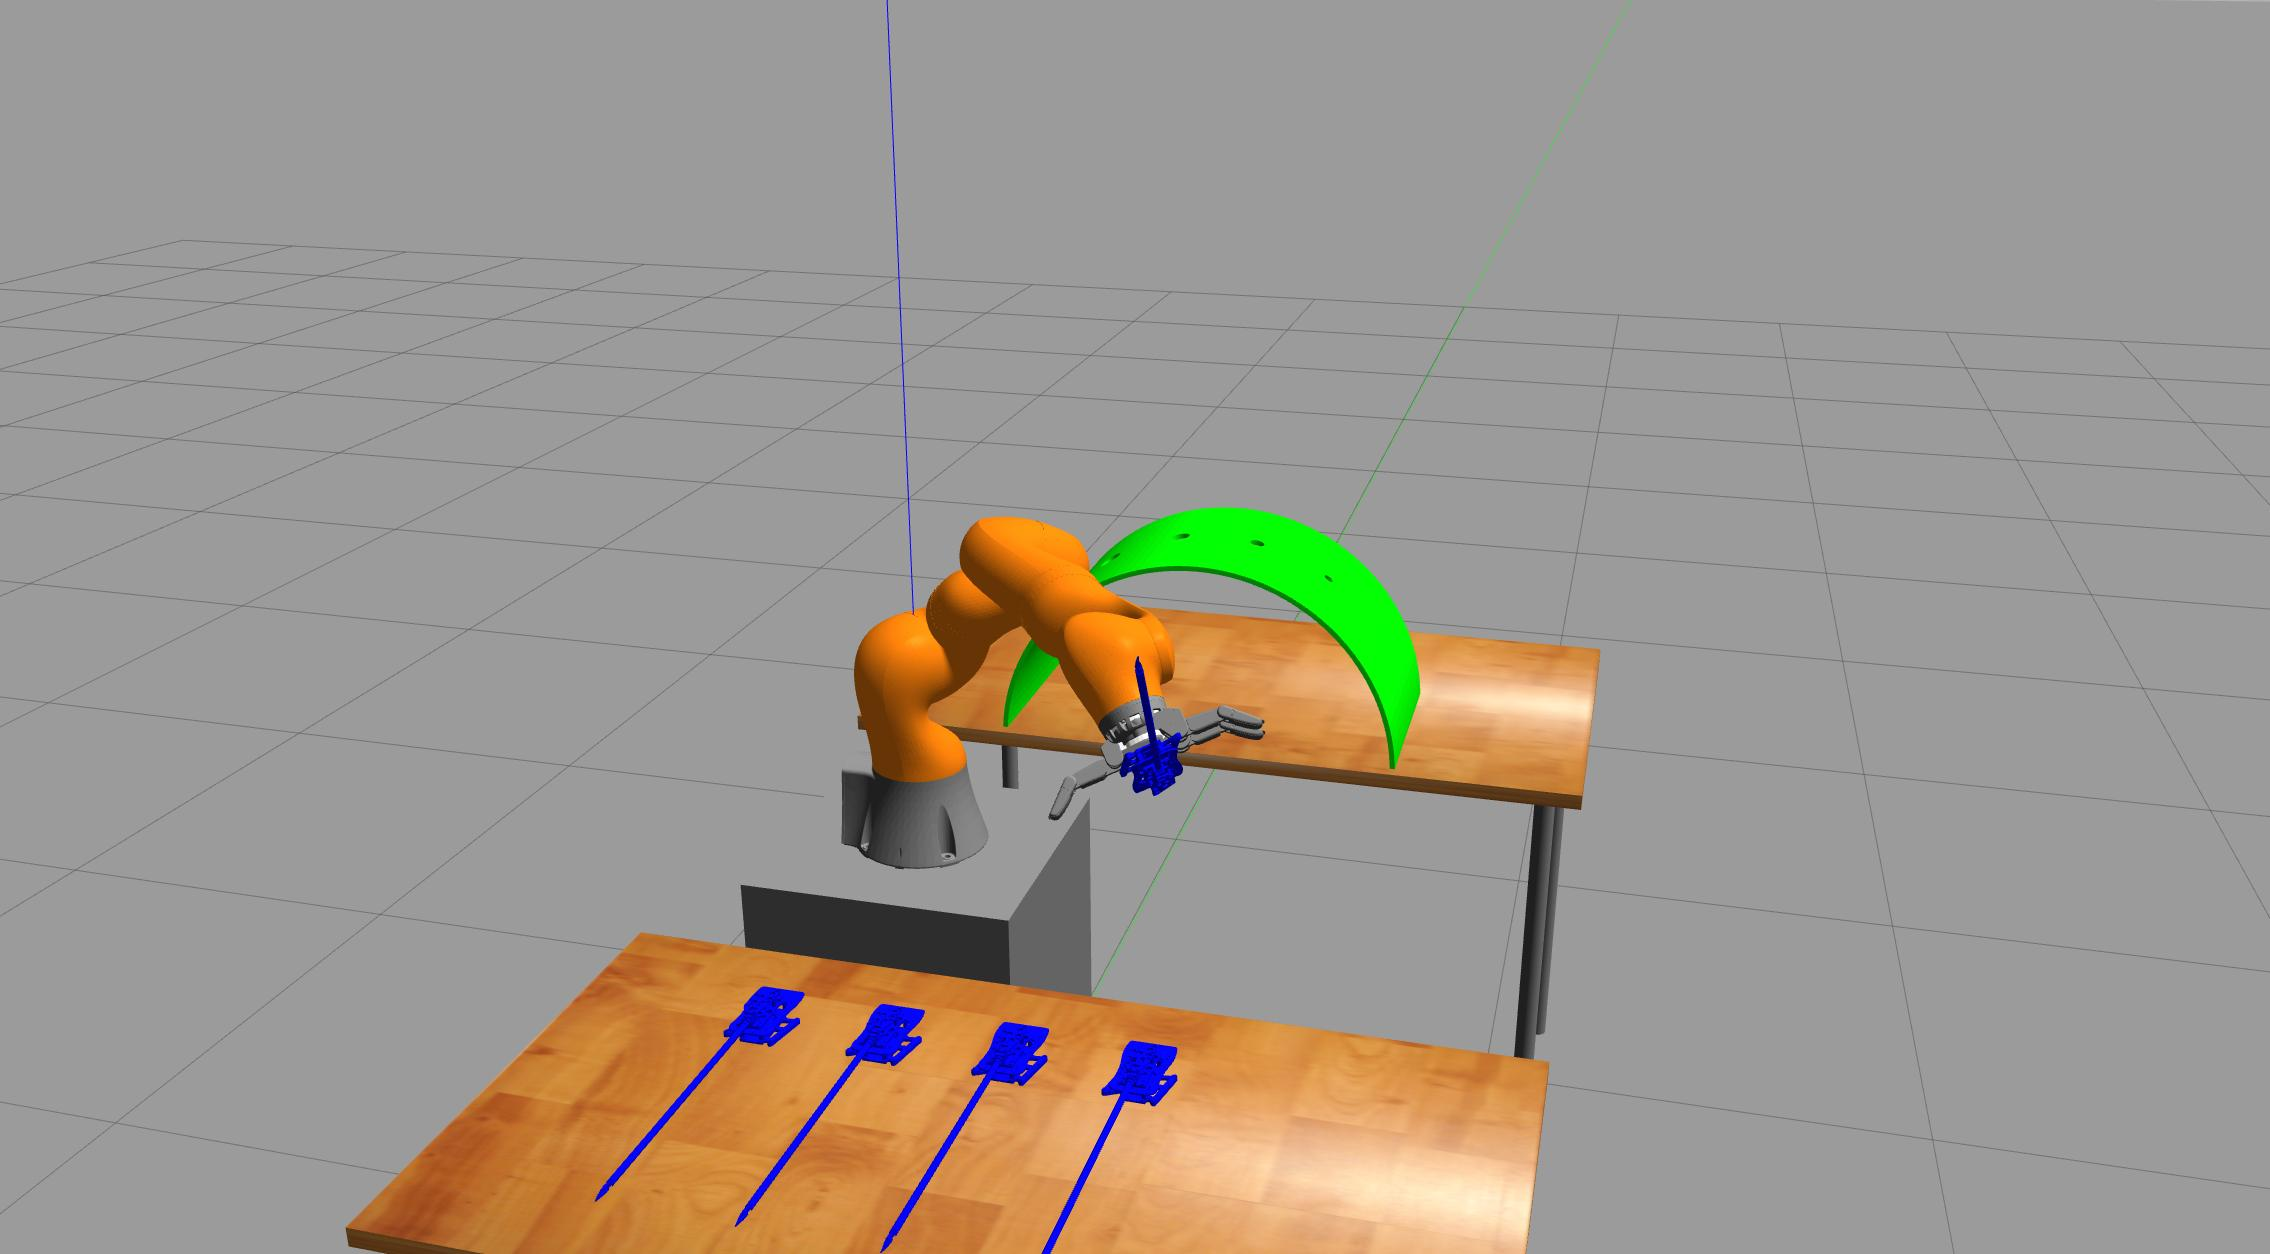
\includegraphics[width=0.3\textwidth]{images/robot_planner1/robot_planner1_3}\\
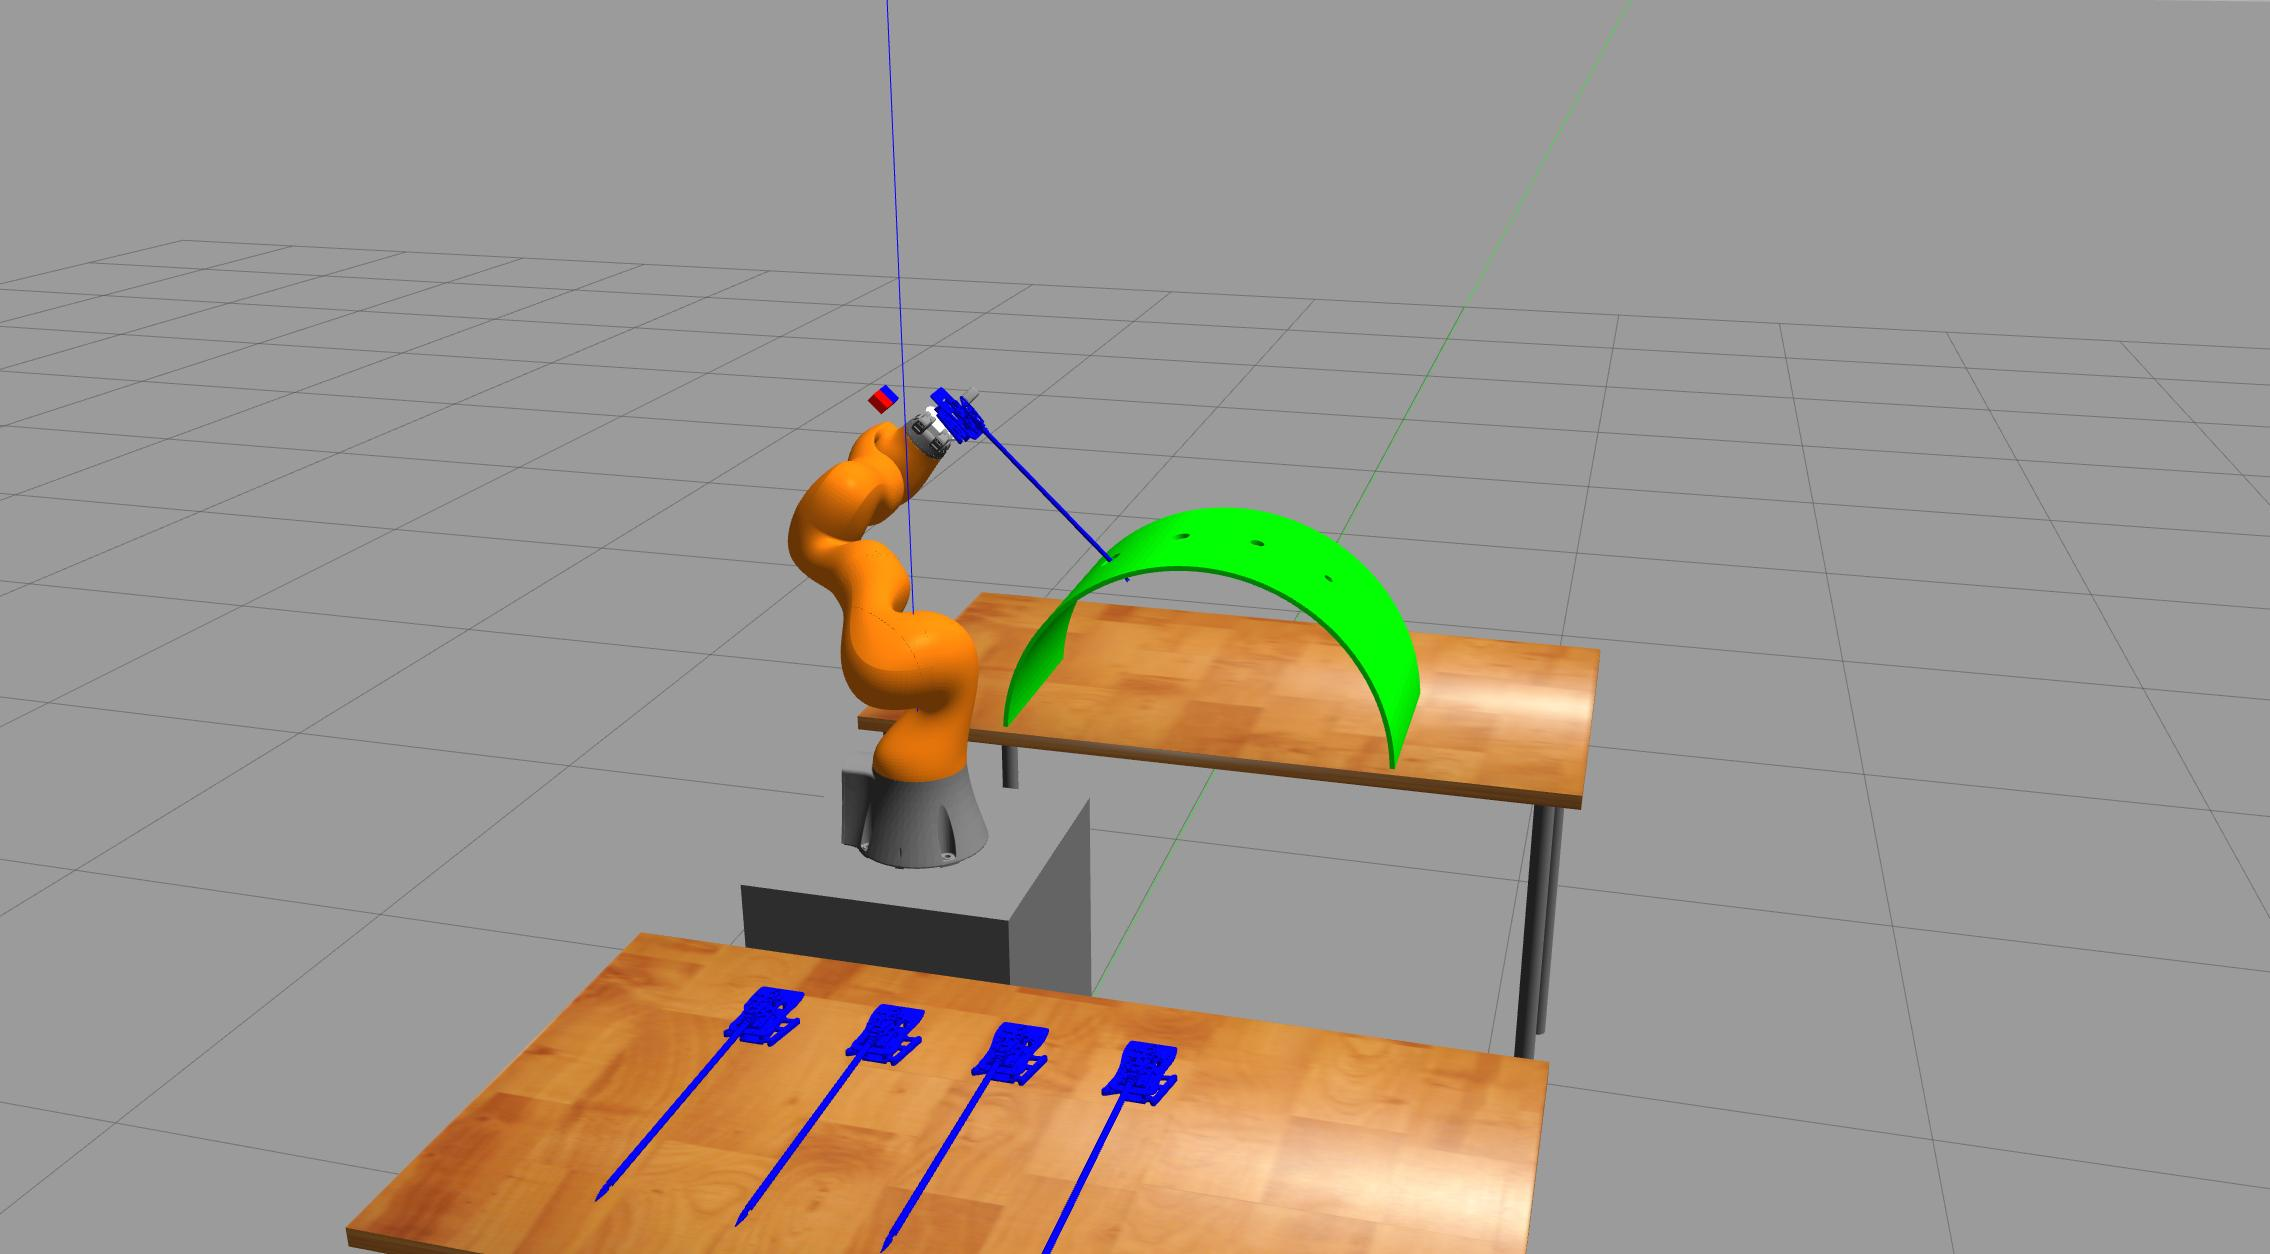
\includegraphics[width=0.3\textwidth]{images/robot_planner1/robot_planner1_4}
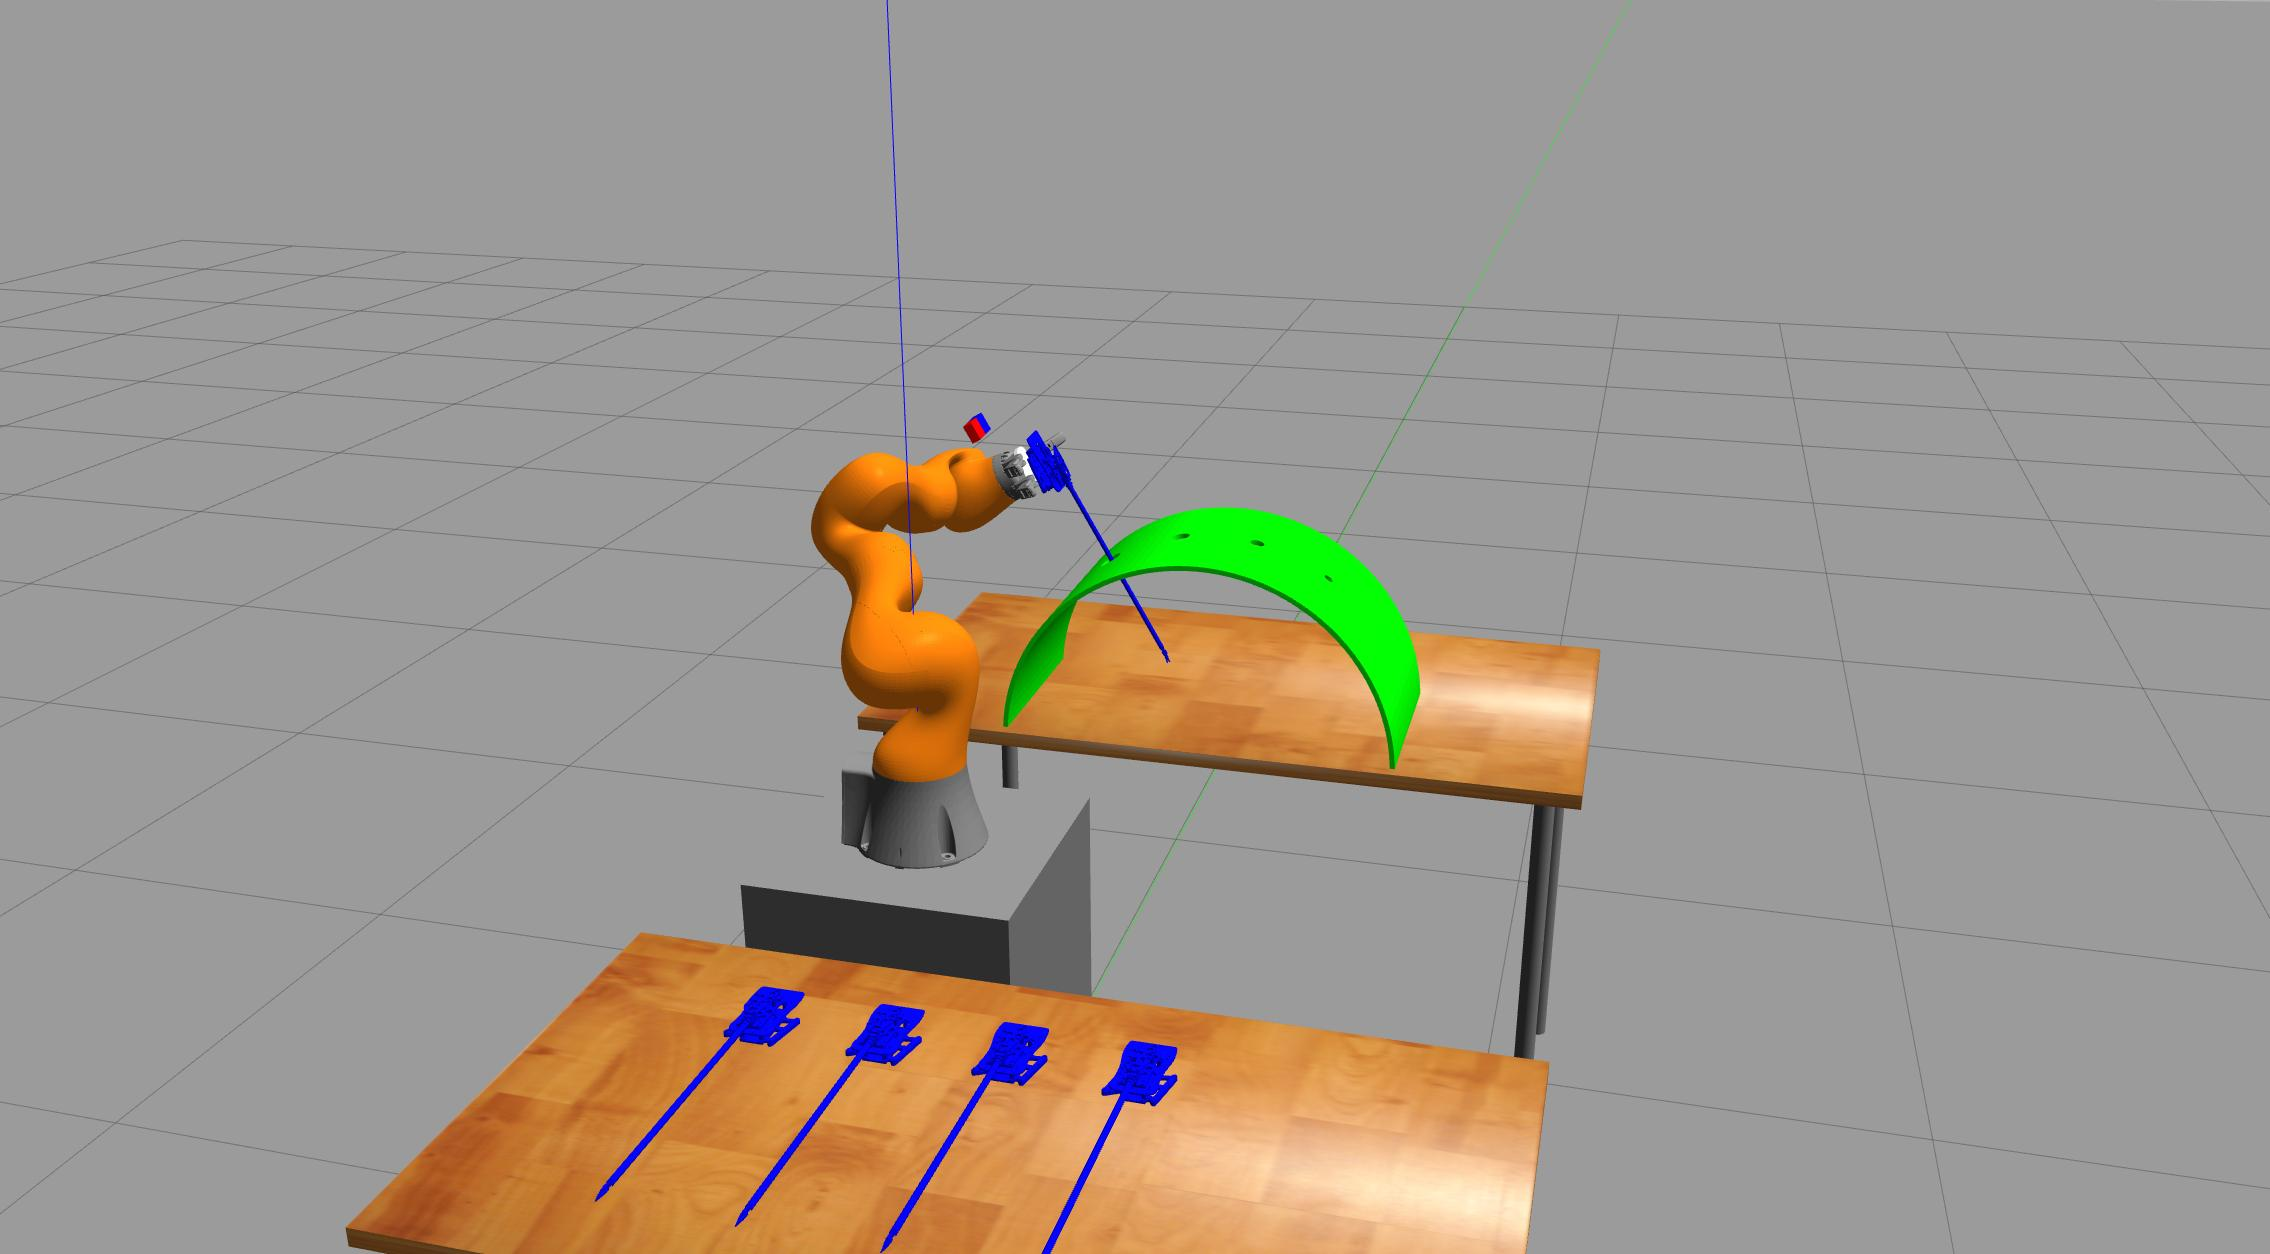
\includegraphics[width=0.3\textwidth]{images/robot_planner1/robot_planner1_5}
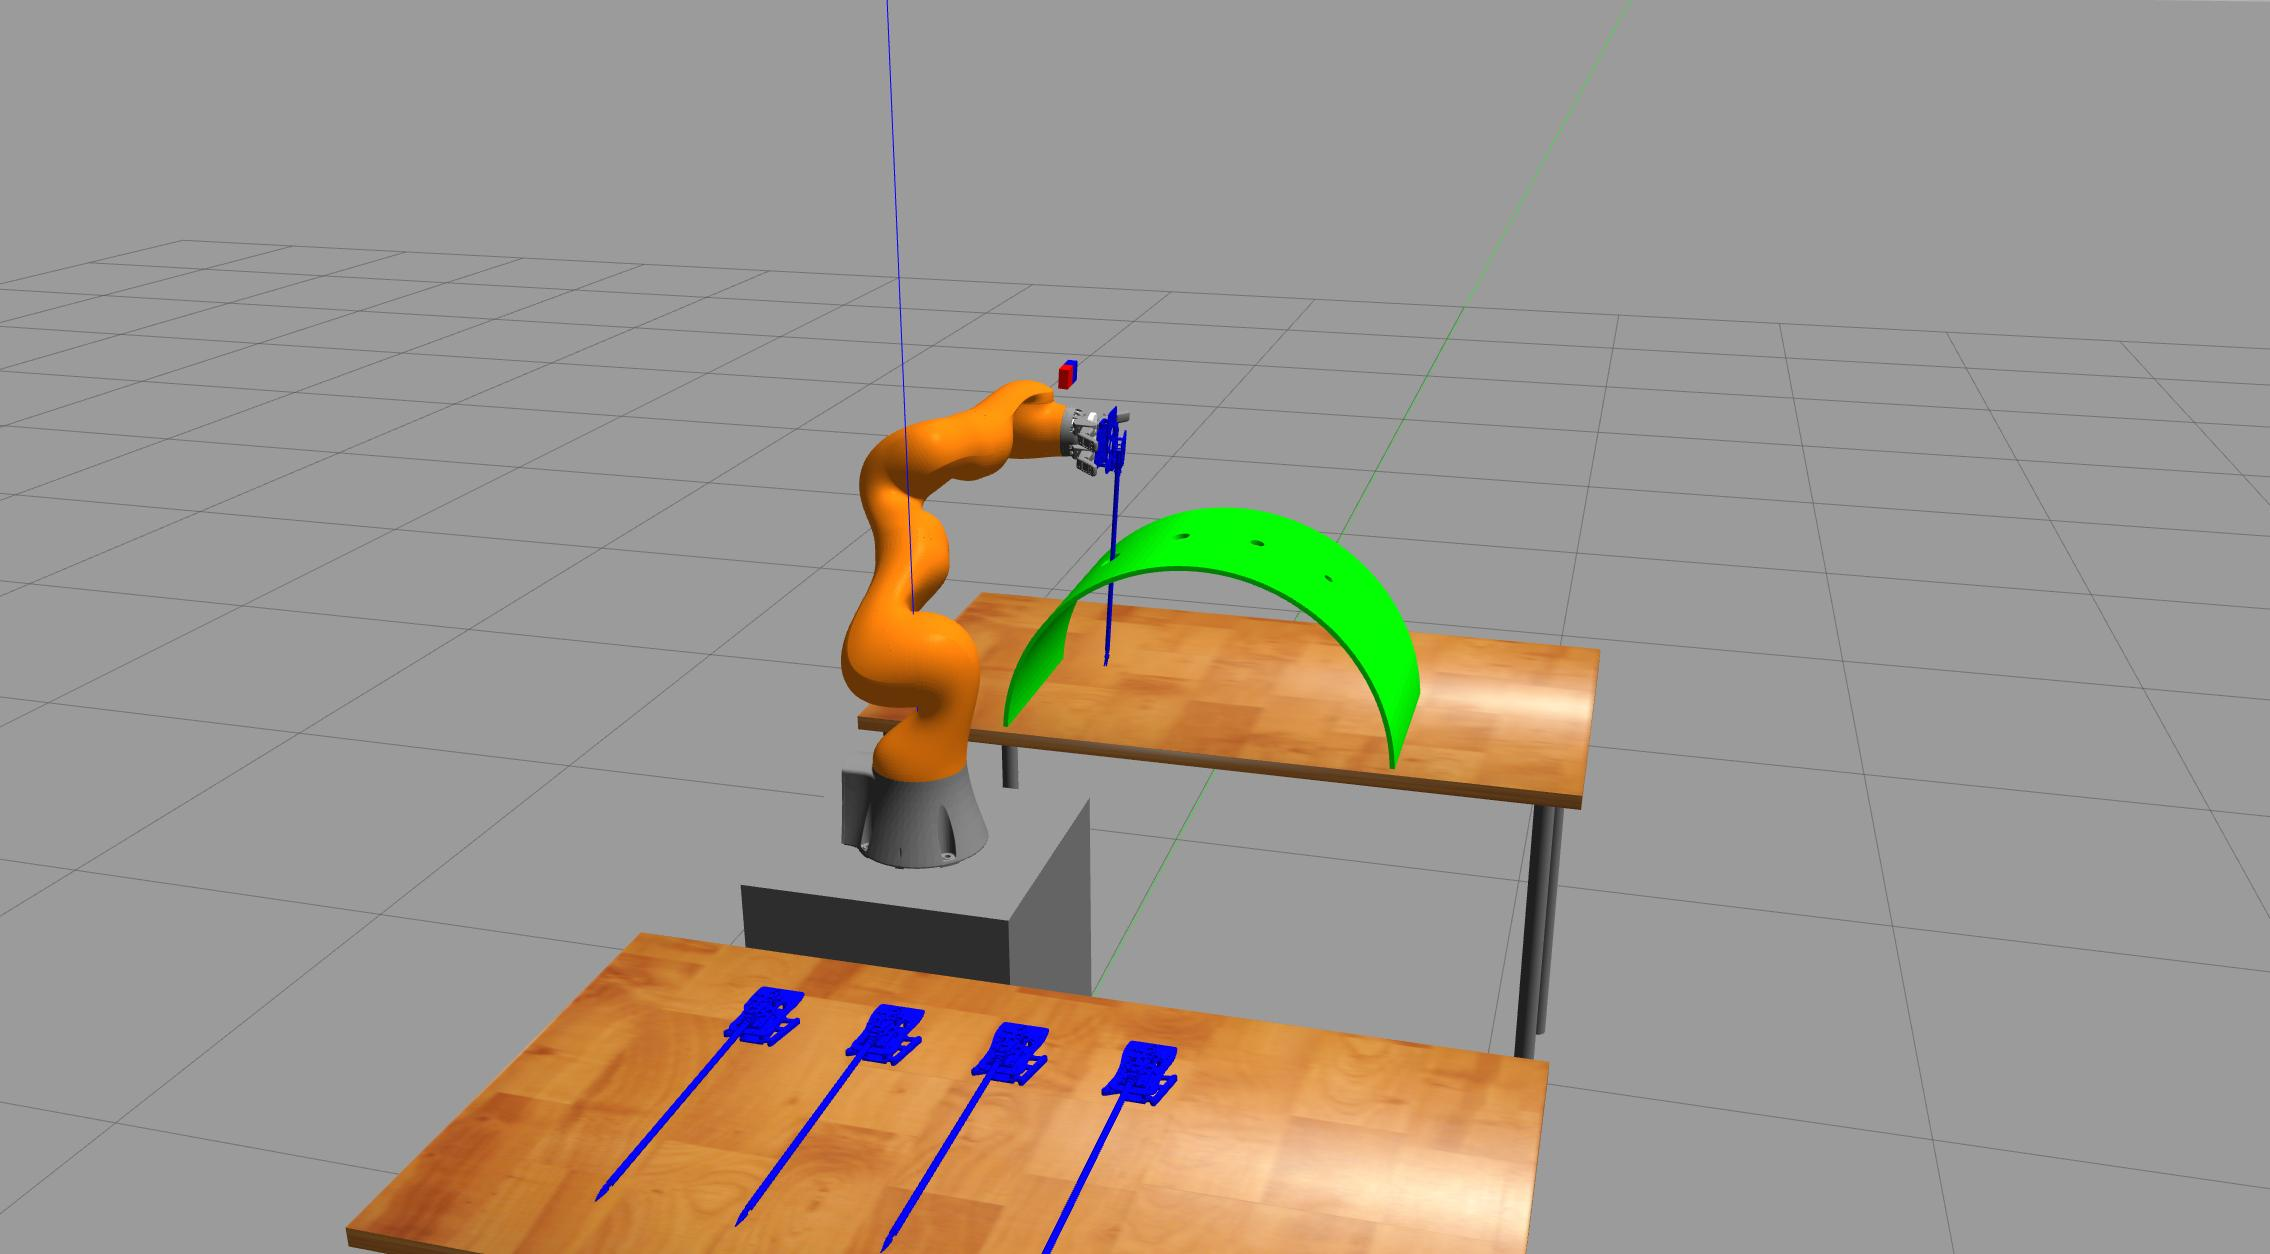
\includegraphics[width=0.3\textwidth]{images/robot_planner1/robot_planner1_6}\\
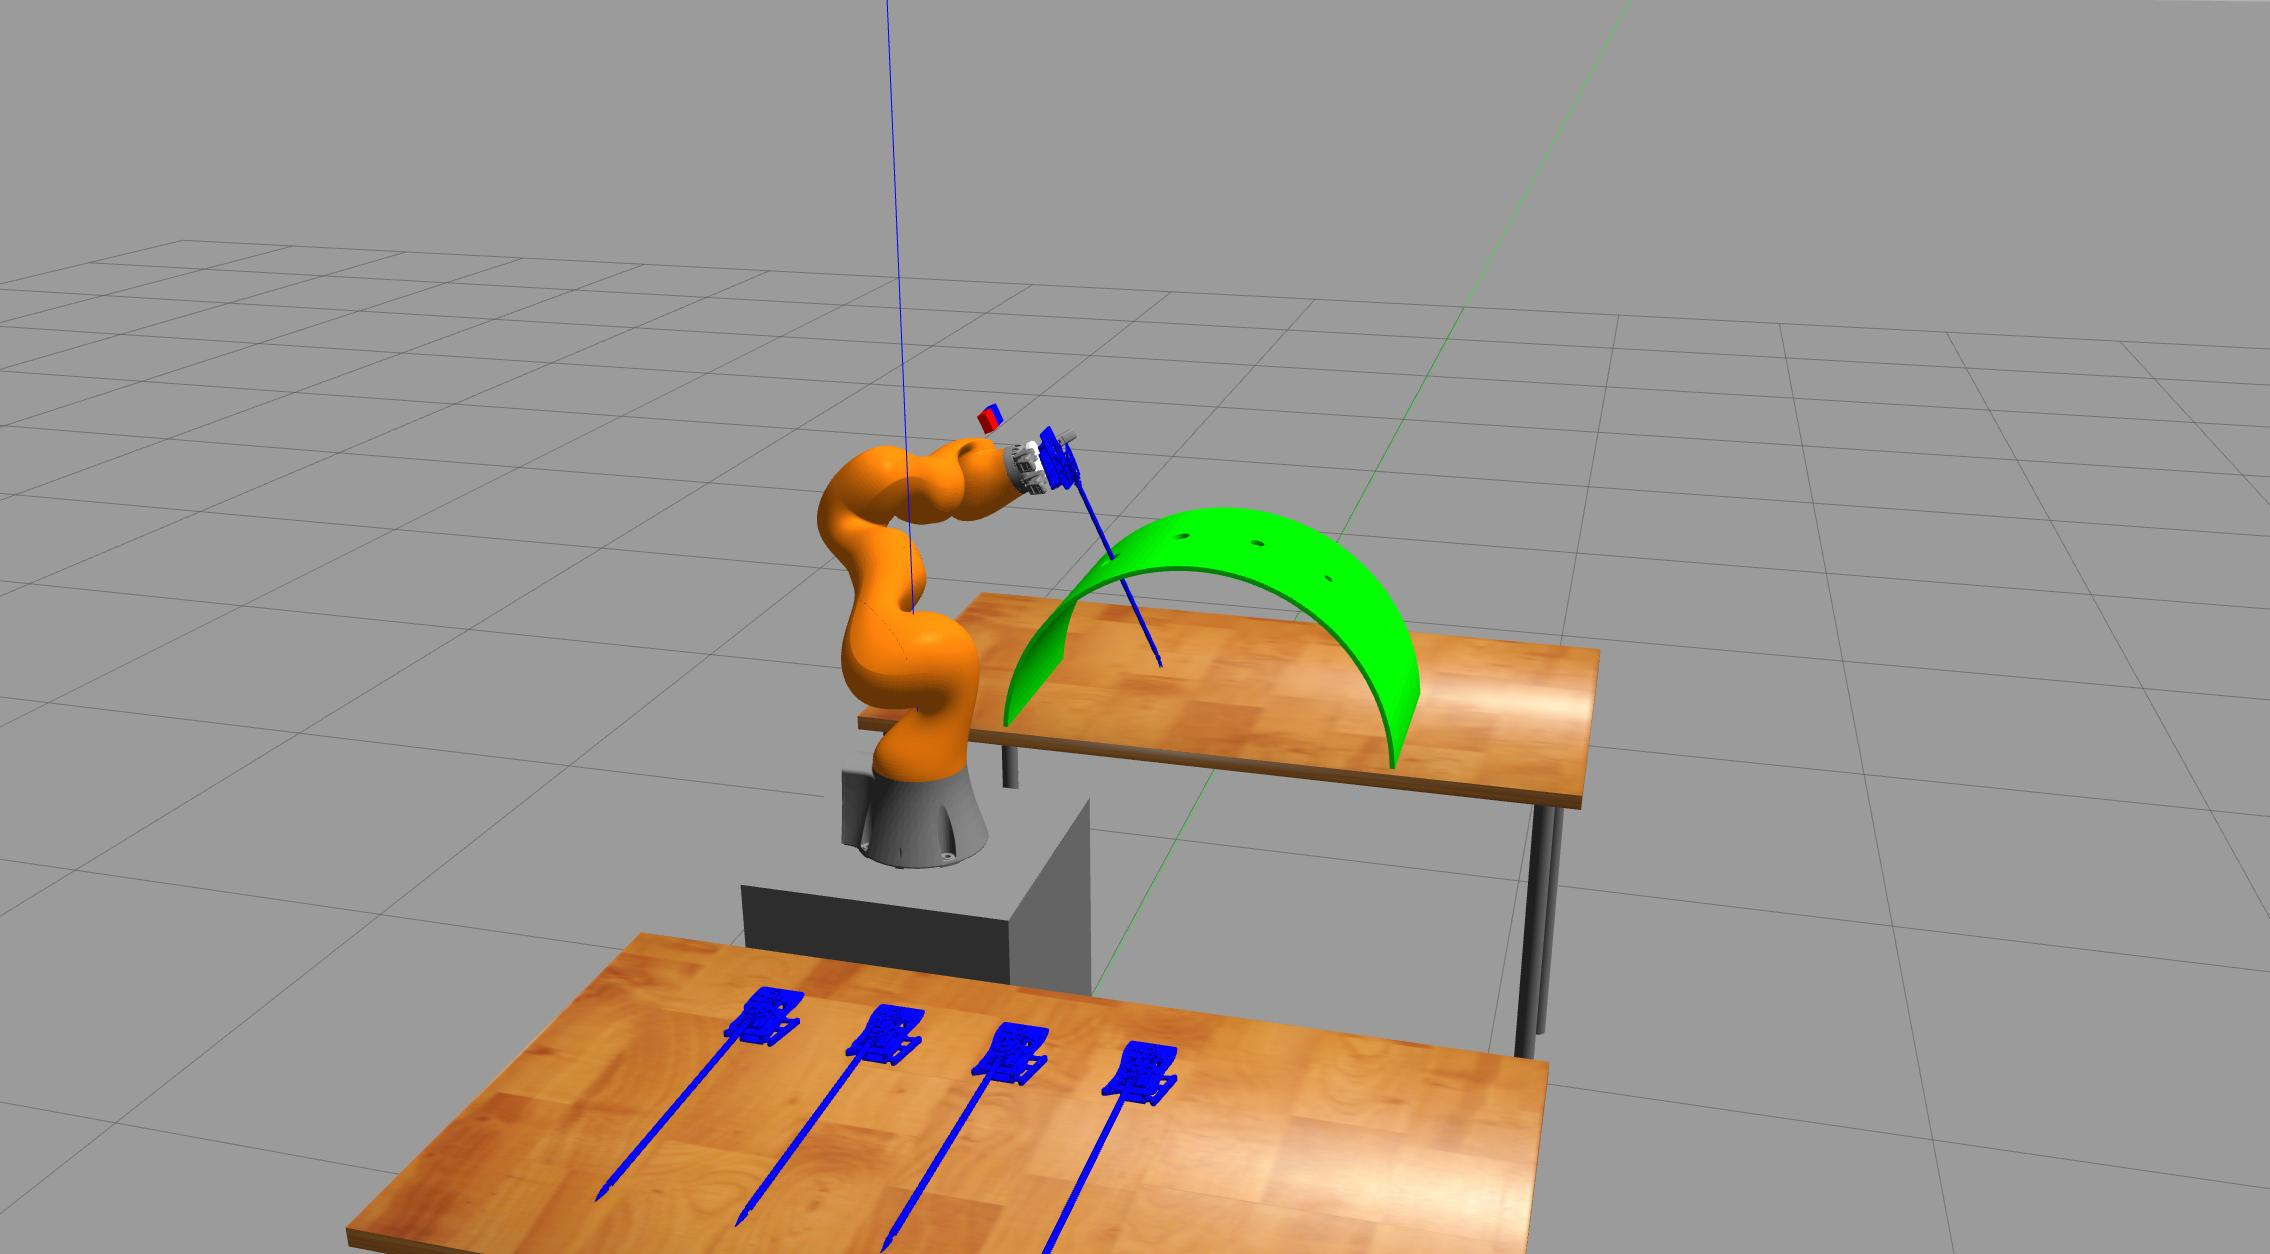
\includegraphics[width=0.3\textwidth]{images/robot_planner1/robot_planner1_7}
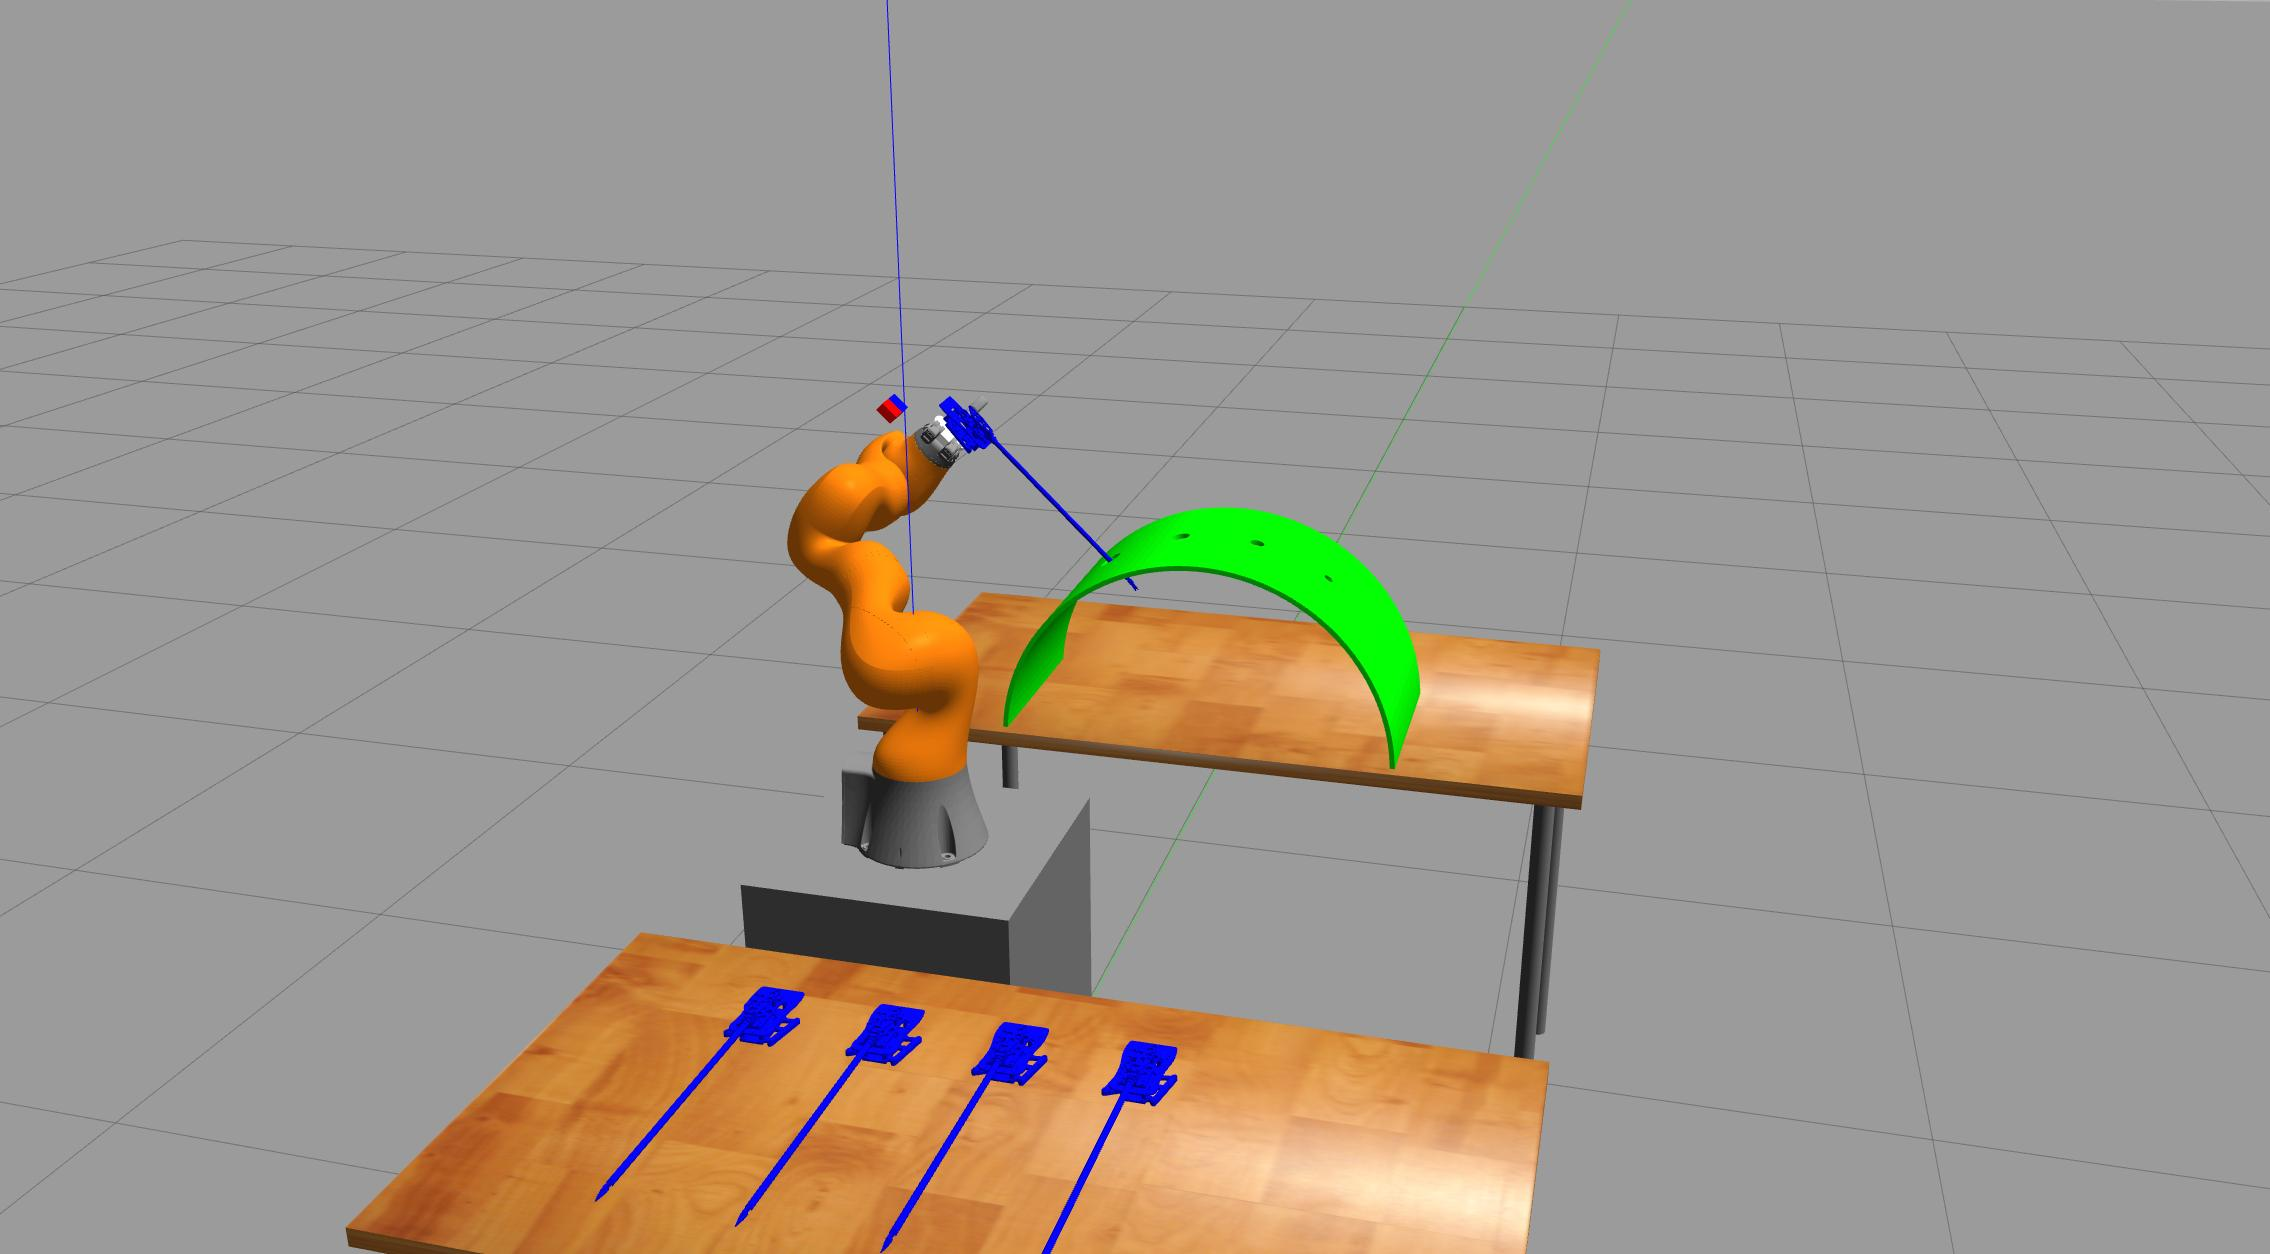
\includegraphics[width=0.3\textwidth]{images/robot_planner1/robot_planner1_8}
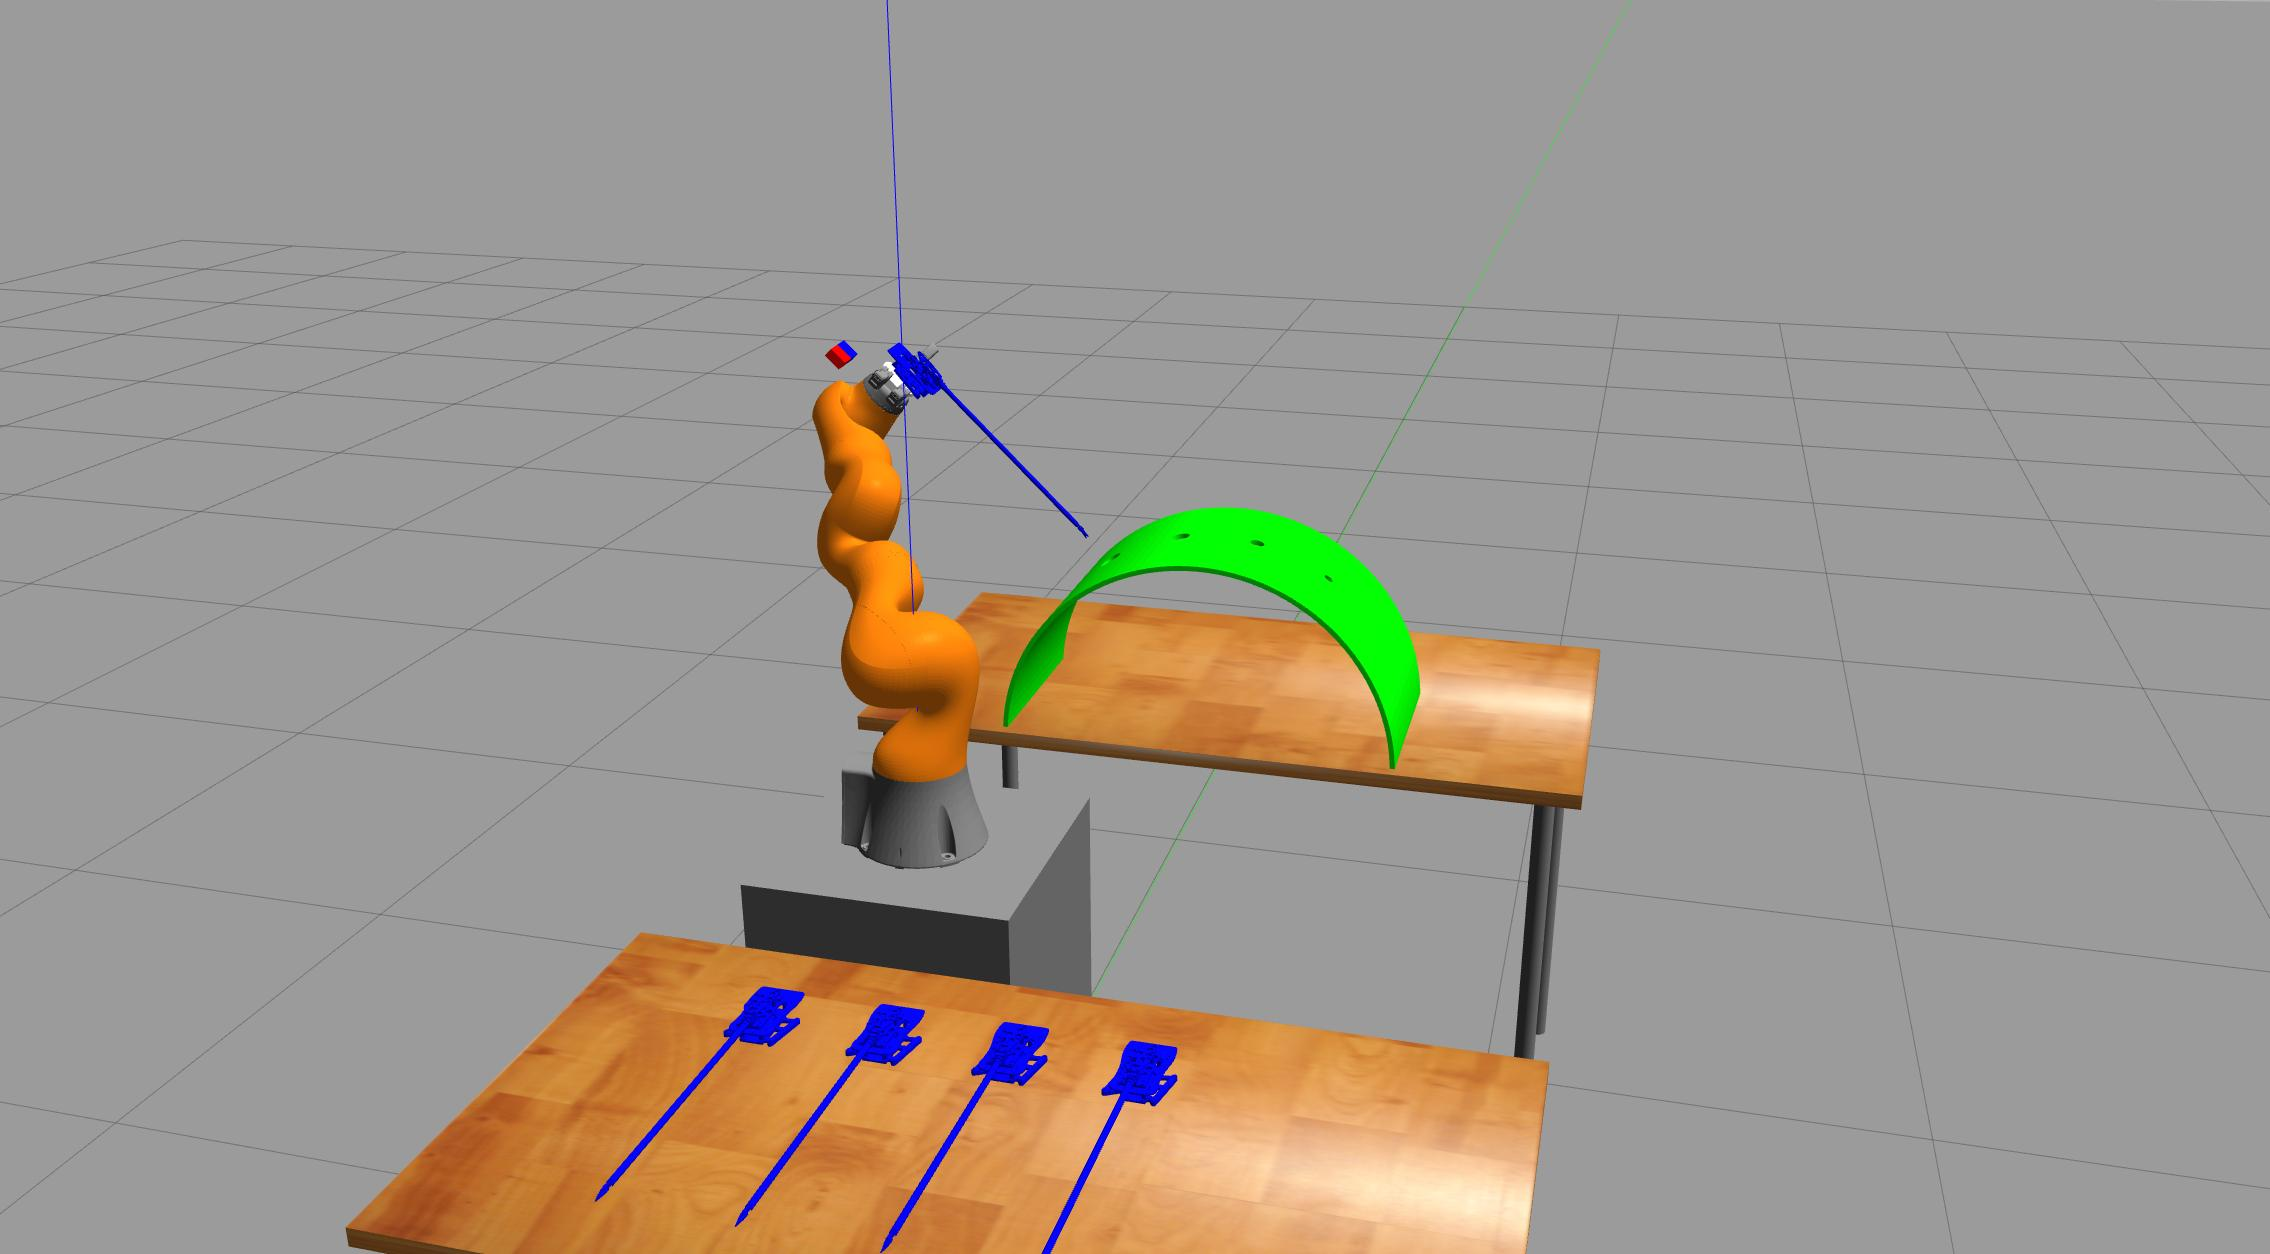
\includegraphics[width=0.3\textwidth]{images/robot_planner1/robot_planner1_9}\\
\caption{Experiment 1:}
\end{figure}
\end{center}


\subsection{Robot Planner 2}

In this experiment, we plan a path such that the robot arm will visit all holes of the mounting dock and will try the insertion movement of the surgical tool.
This experiment is very useful, because it shows whether all holes of the mounting dock are \textbf{reachable} (inside the robot's work space) and if so, how 
\textbf{dexterous} the robot will be in pivoting around each hole, i.e. how free the robot arm is to execute pivot motions.

\begin{center}
\begin{figure}[H]
\centering
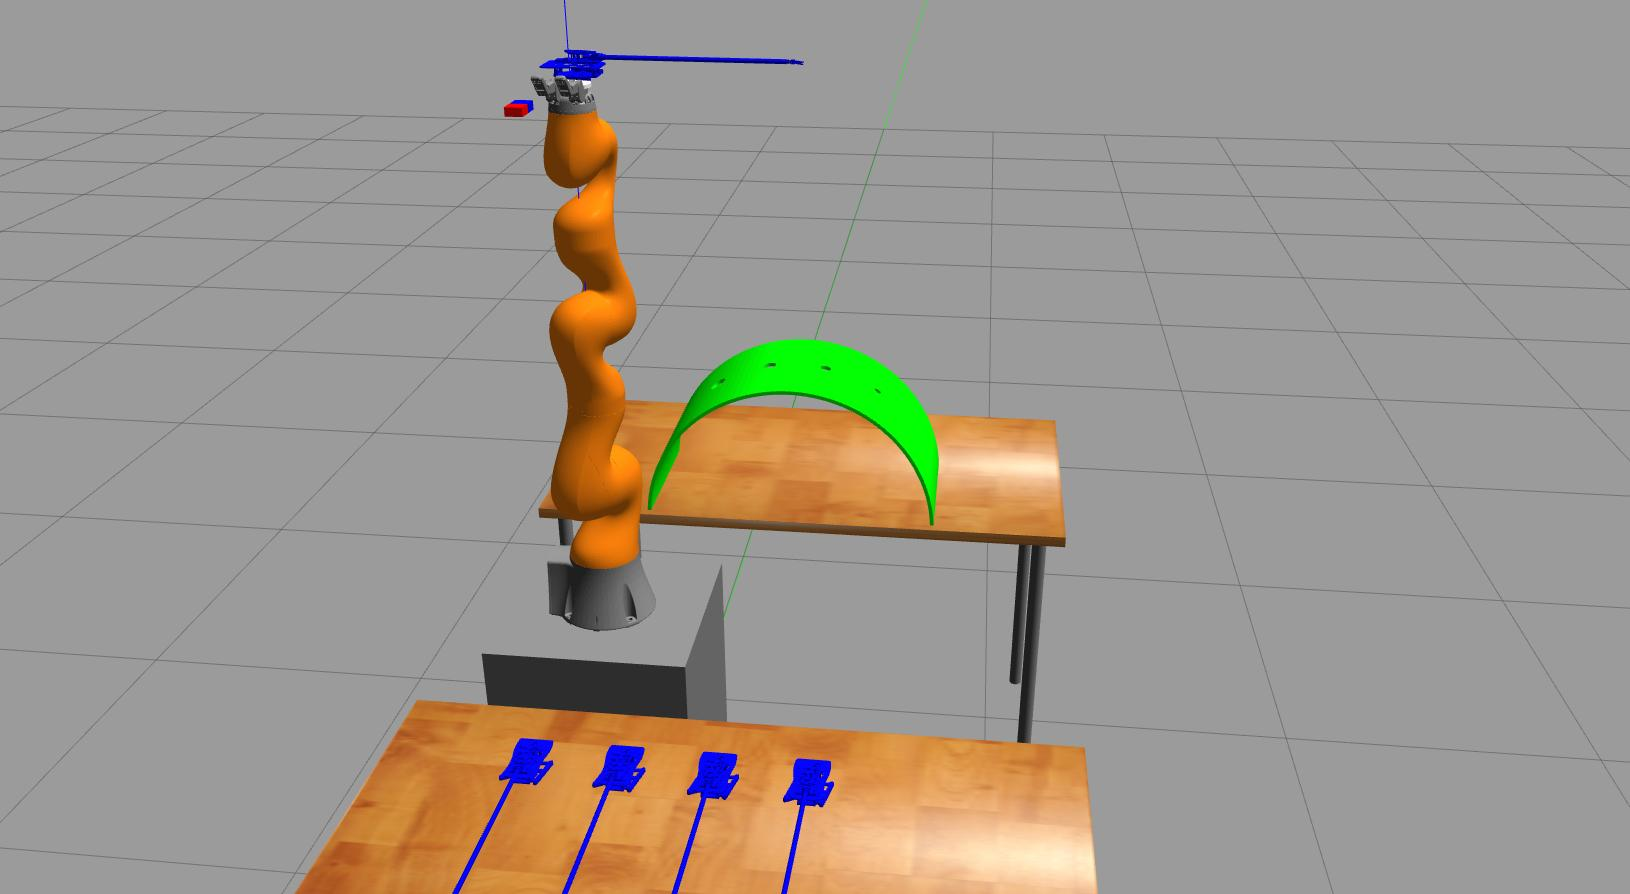
\includegraphics[width=0.3\textwidth]{images/robot_planner2/robot_planner2_1}
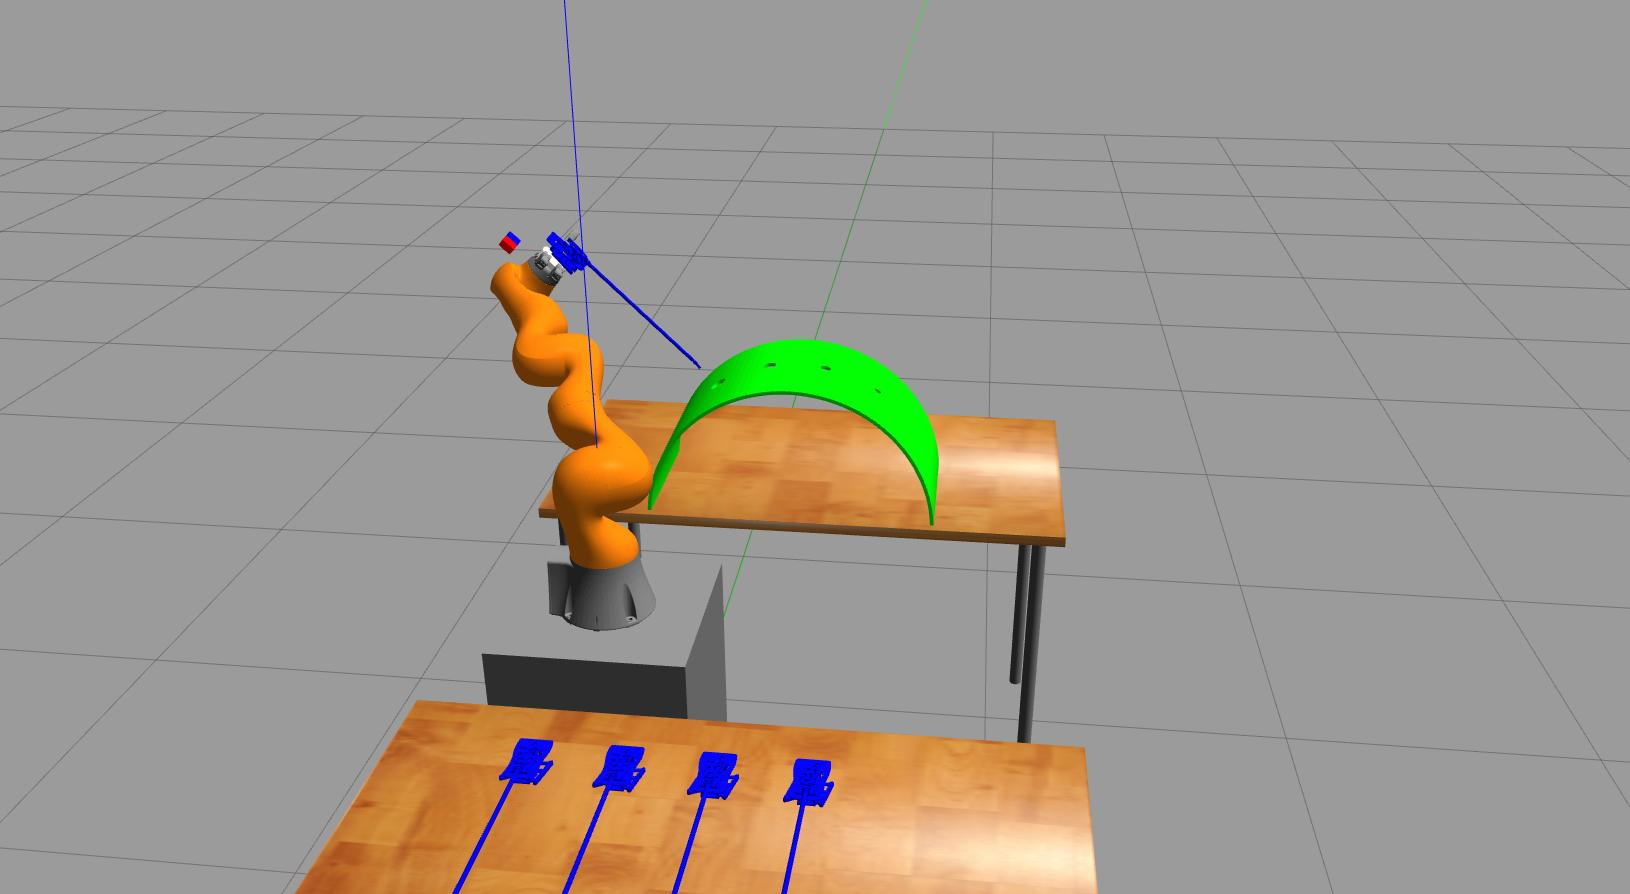
\includegraphics[width=0.3\textwidth]{images/robot_planner2/robot_planner2_2}
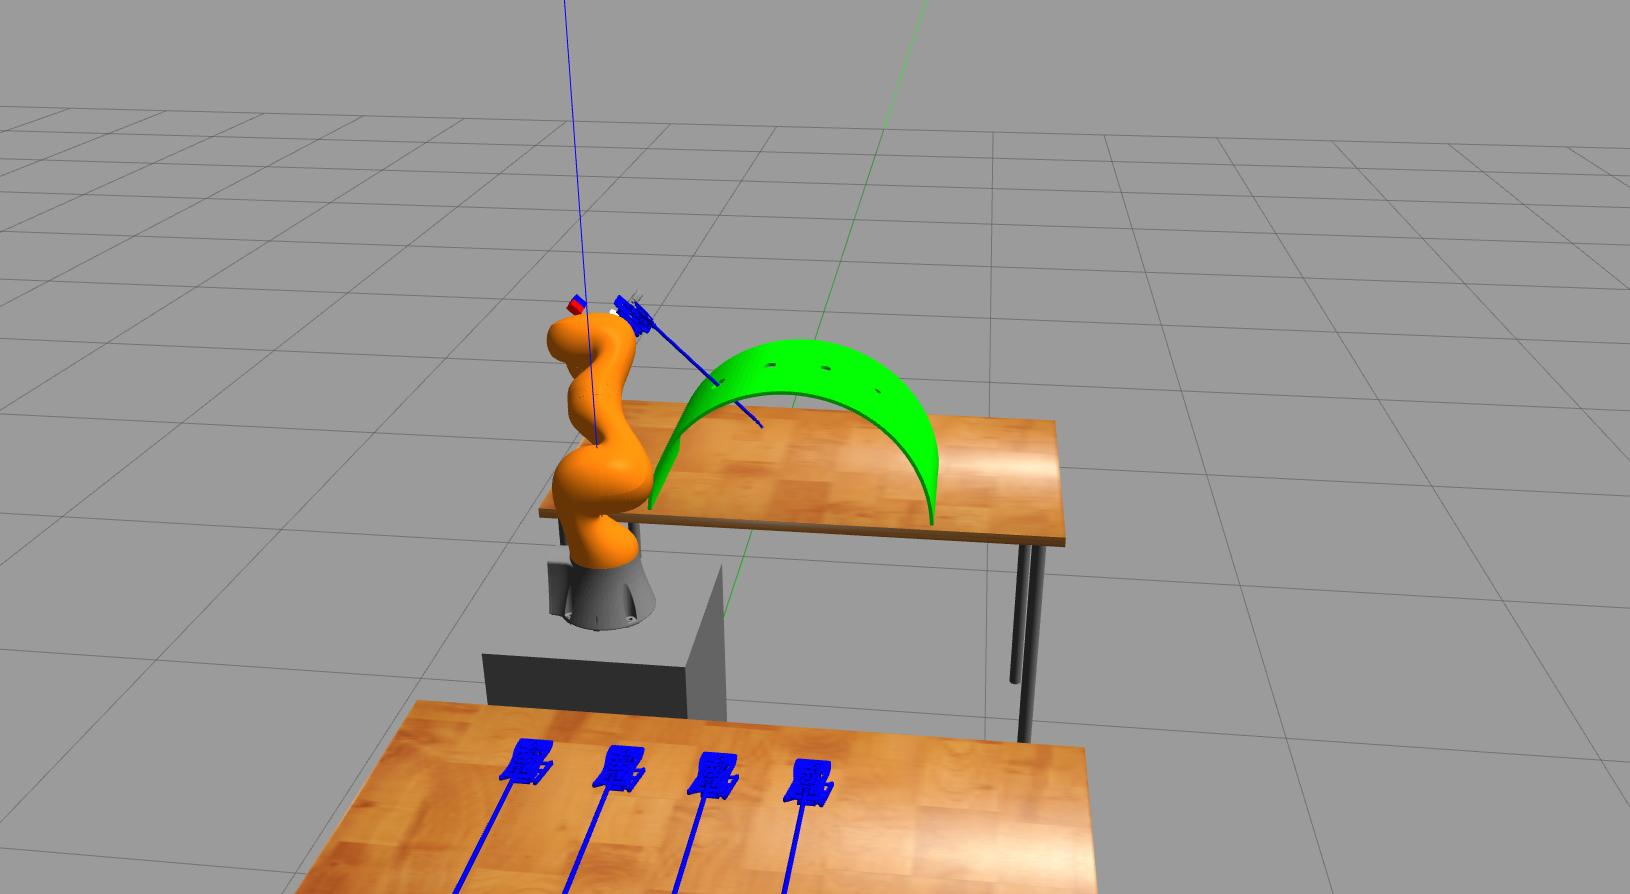
\includegraphics[width=0.3\textwidth]{images/robot_planner2/robot_planner2_3}\\
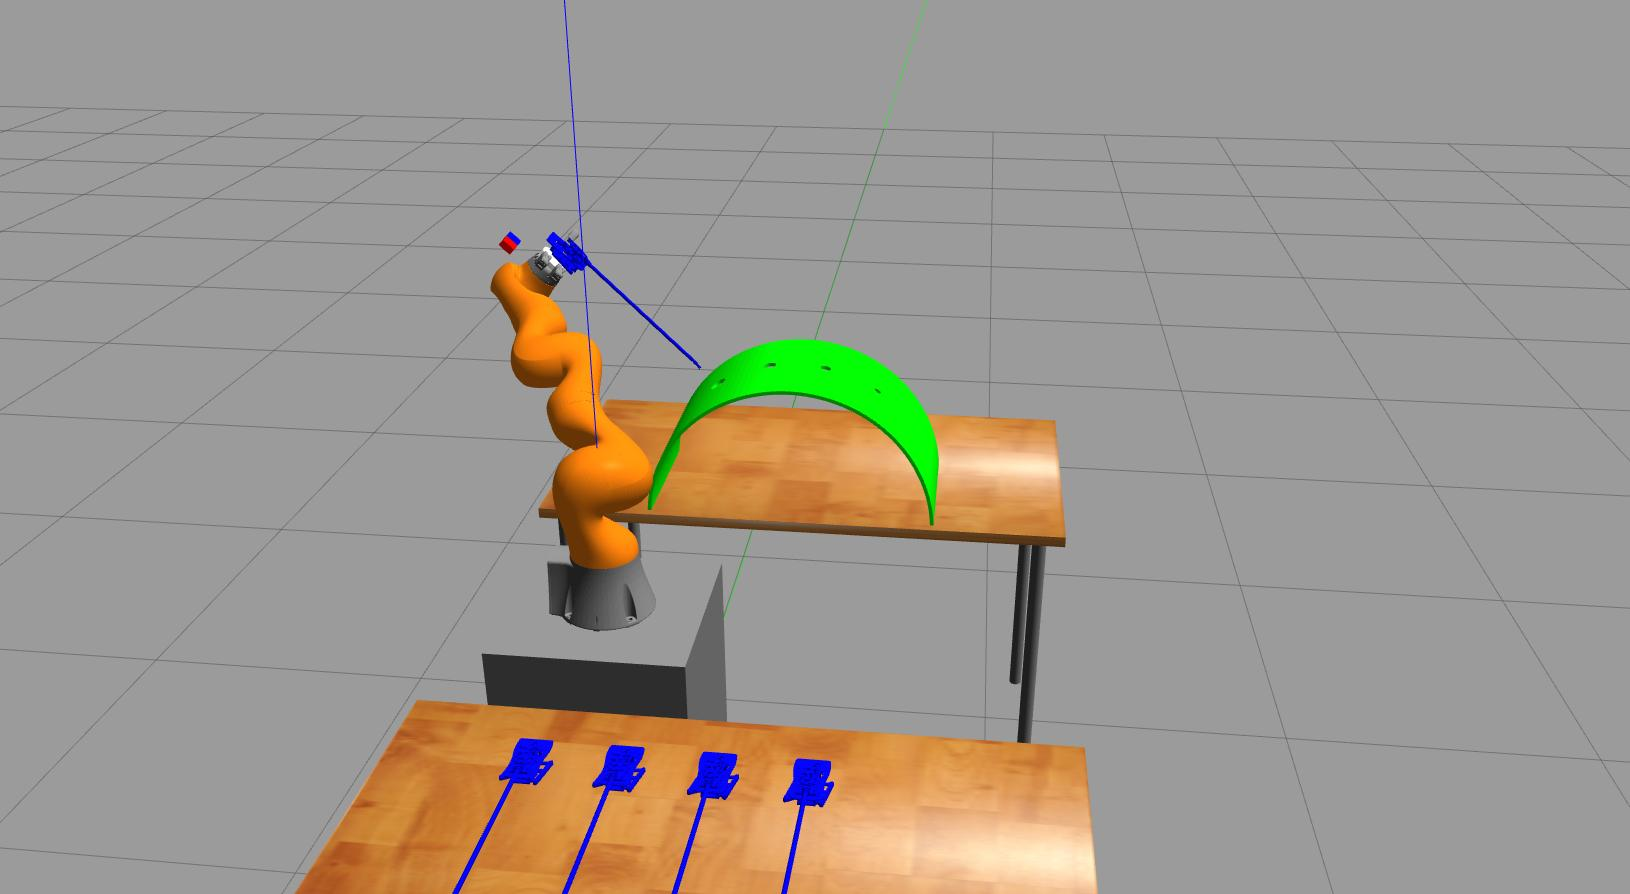
\includegraphics[width=0.3\textwidth]{images/robot_planner2/robot_planner2_4}
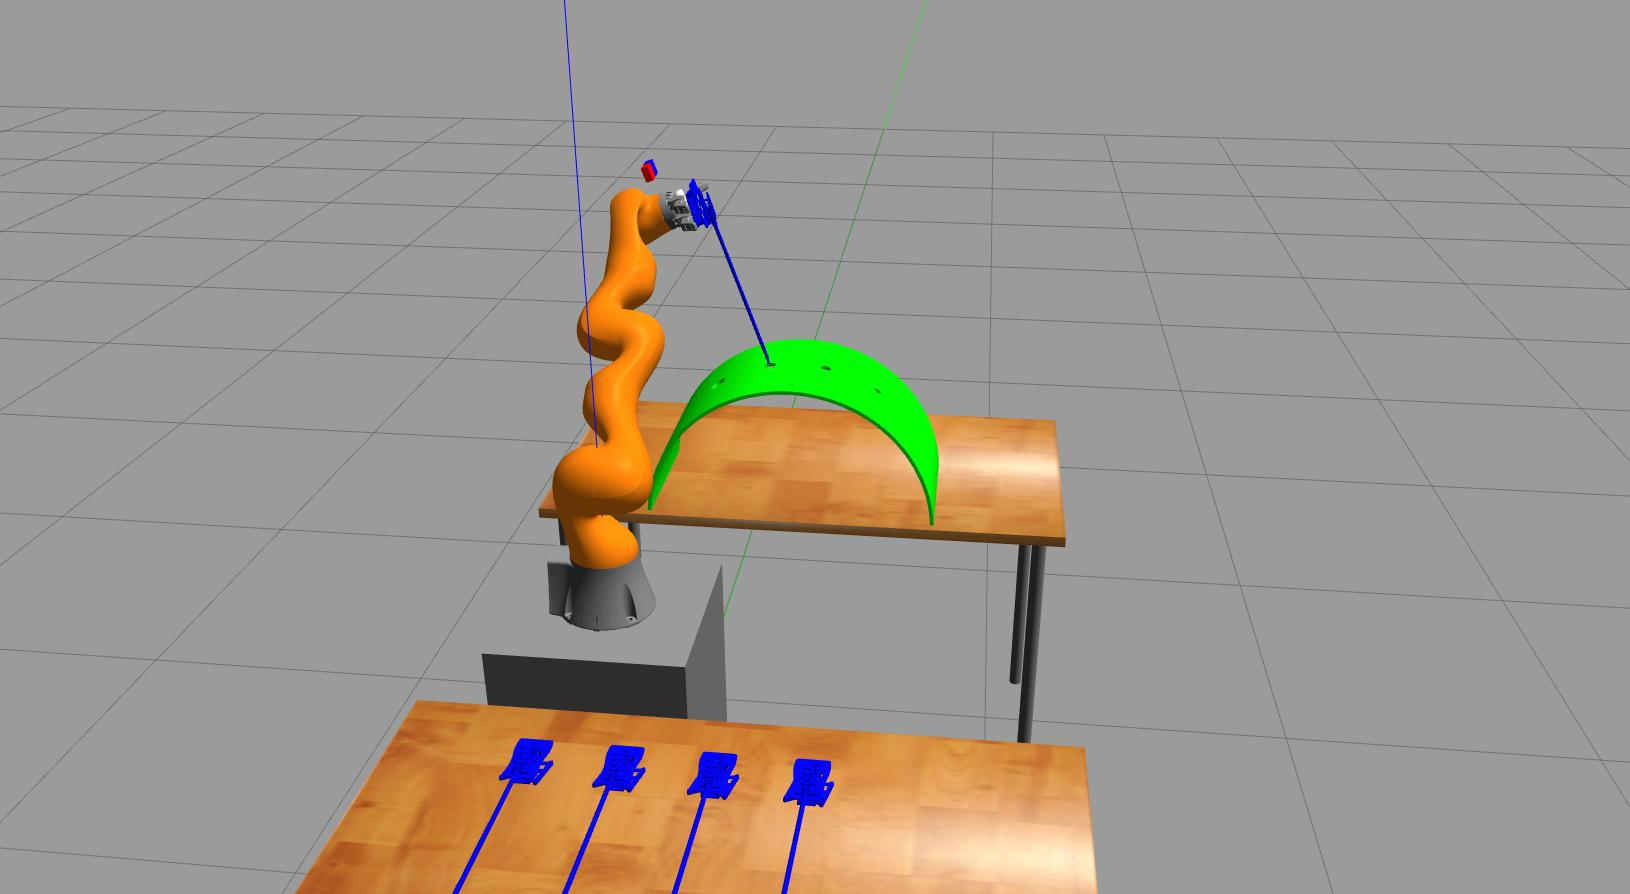
\includegraphics[width=0.3\textwidth]{images/robot_planner2/robot_planner2_5}
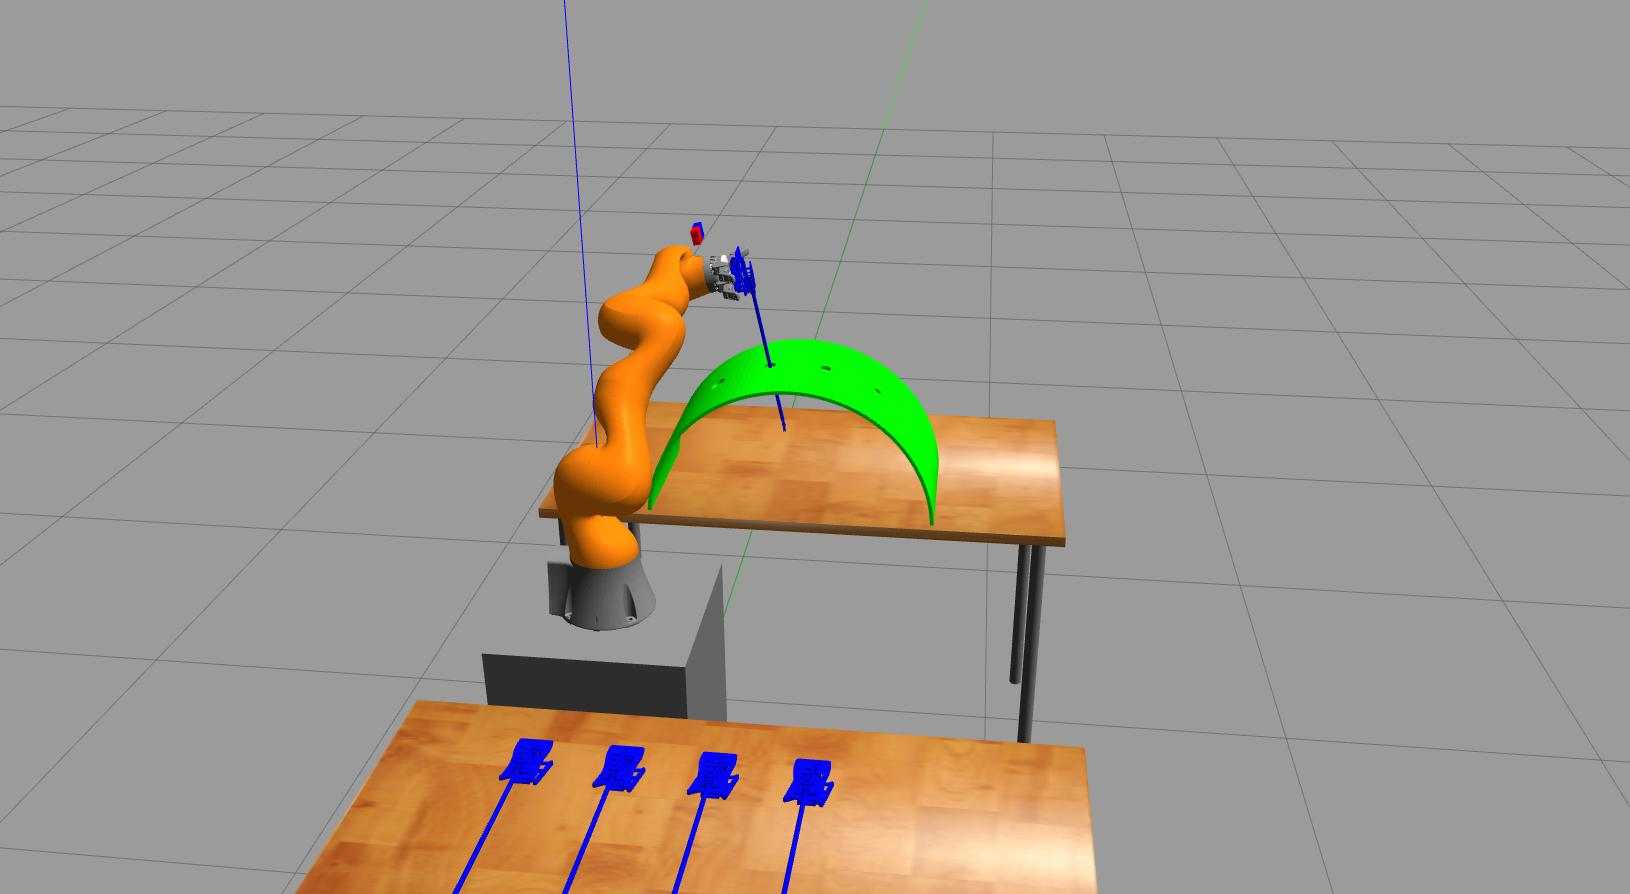
\includegraphics[width=0.3\textwidth]{images/robot_planner2/robot_planner2_6}\\
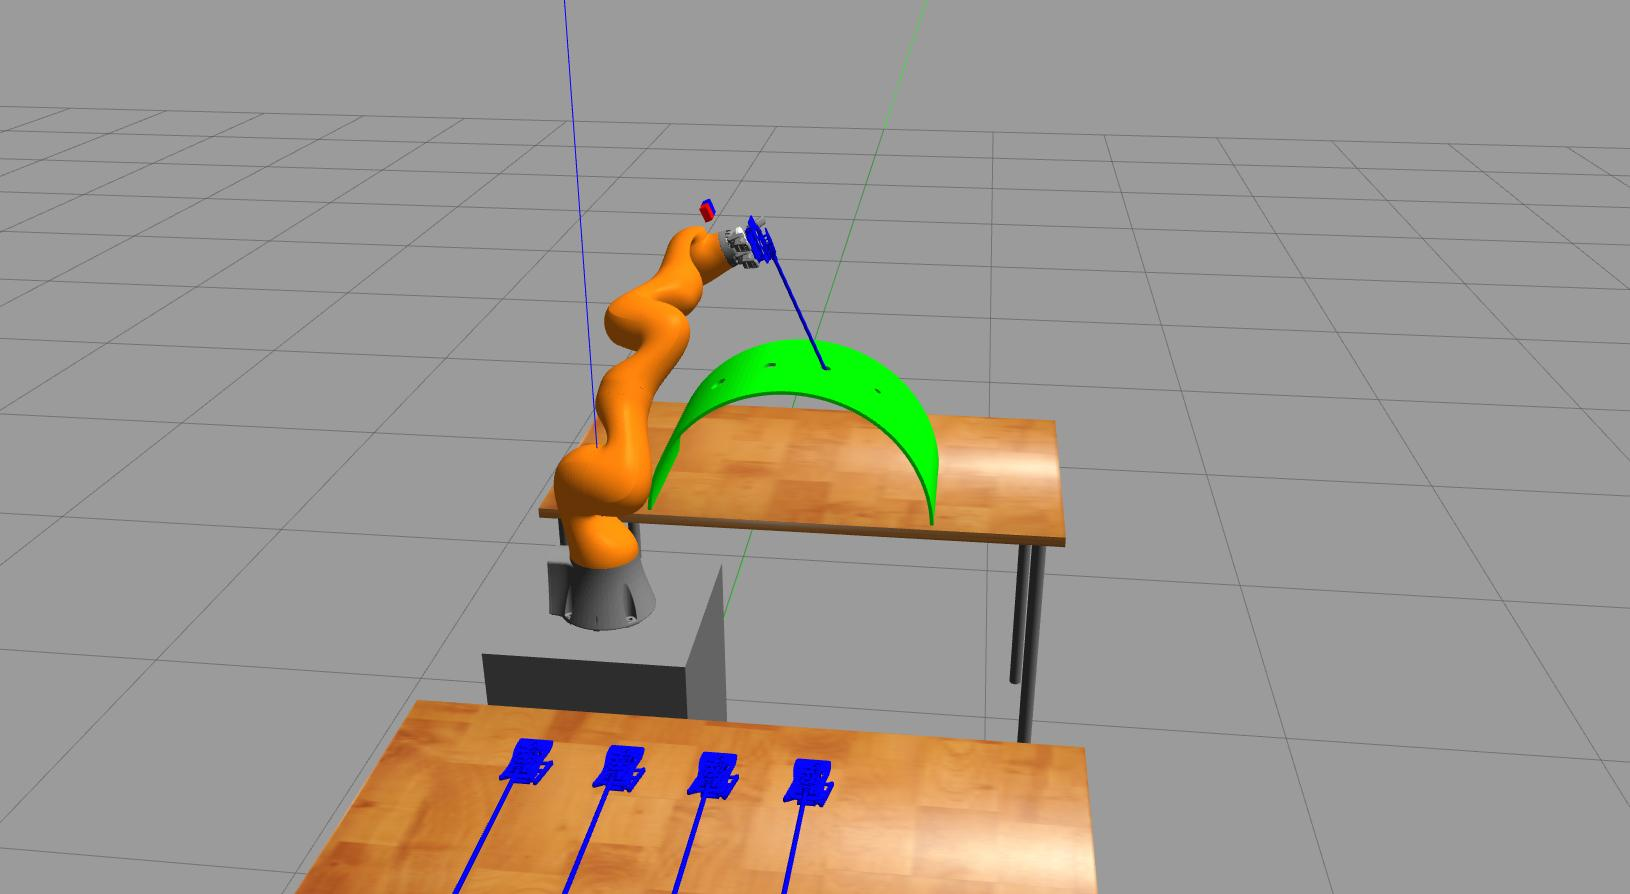
\includegraphics[width=0.3\textwidth]{images/robot_planner2/robot_planner2_7}
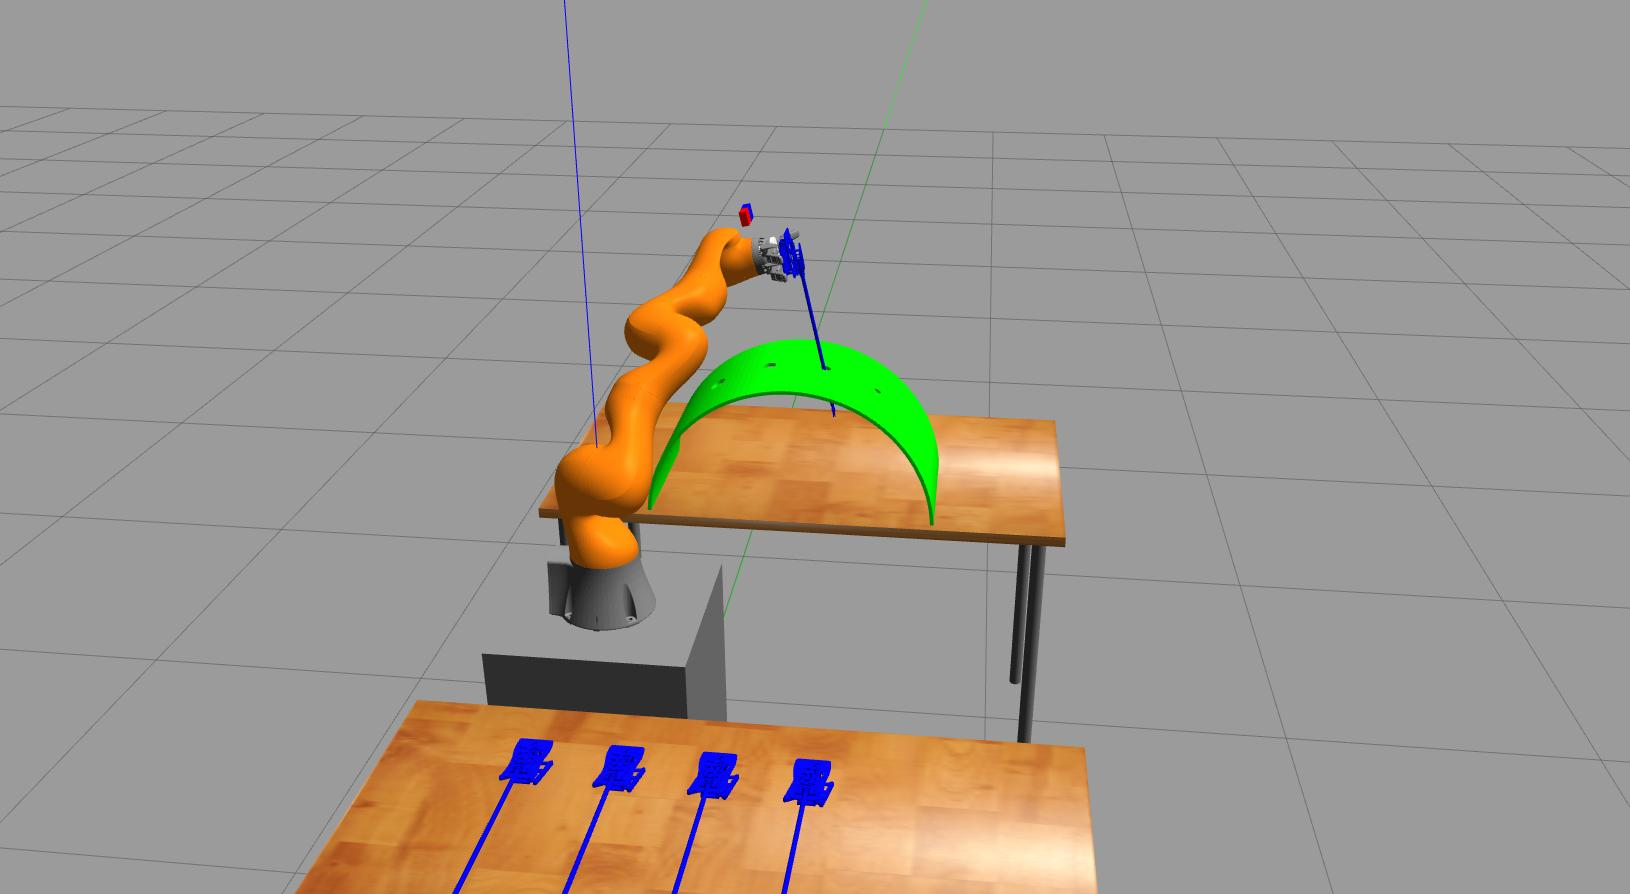
\includegraphics[width=0.3\textwidth]{images/robot_planner2/robot_planner2_8}\\
\caption{Experiment 2a:}
\label{experiment-robot-planner2a}
\end{figure}
\end{center}

To overcome the reachability issue shown in Figure \ref{experiment-robot-planner2a}, the algorithm was repeated, but this time using a different simulation layout 
in Gazebo, in which the mounting dock is closer to the robot and in front of it. This new layout enables the robot to reach all mounting holes with ease and 
with sufficient dexterity, the robot is free to pivot around.

\begin{center}
\begin{figure}[H]
\centering
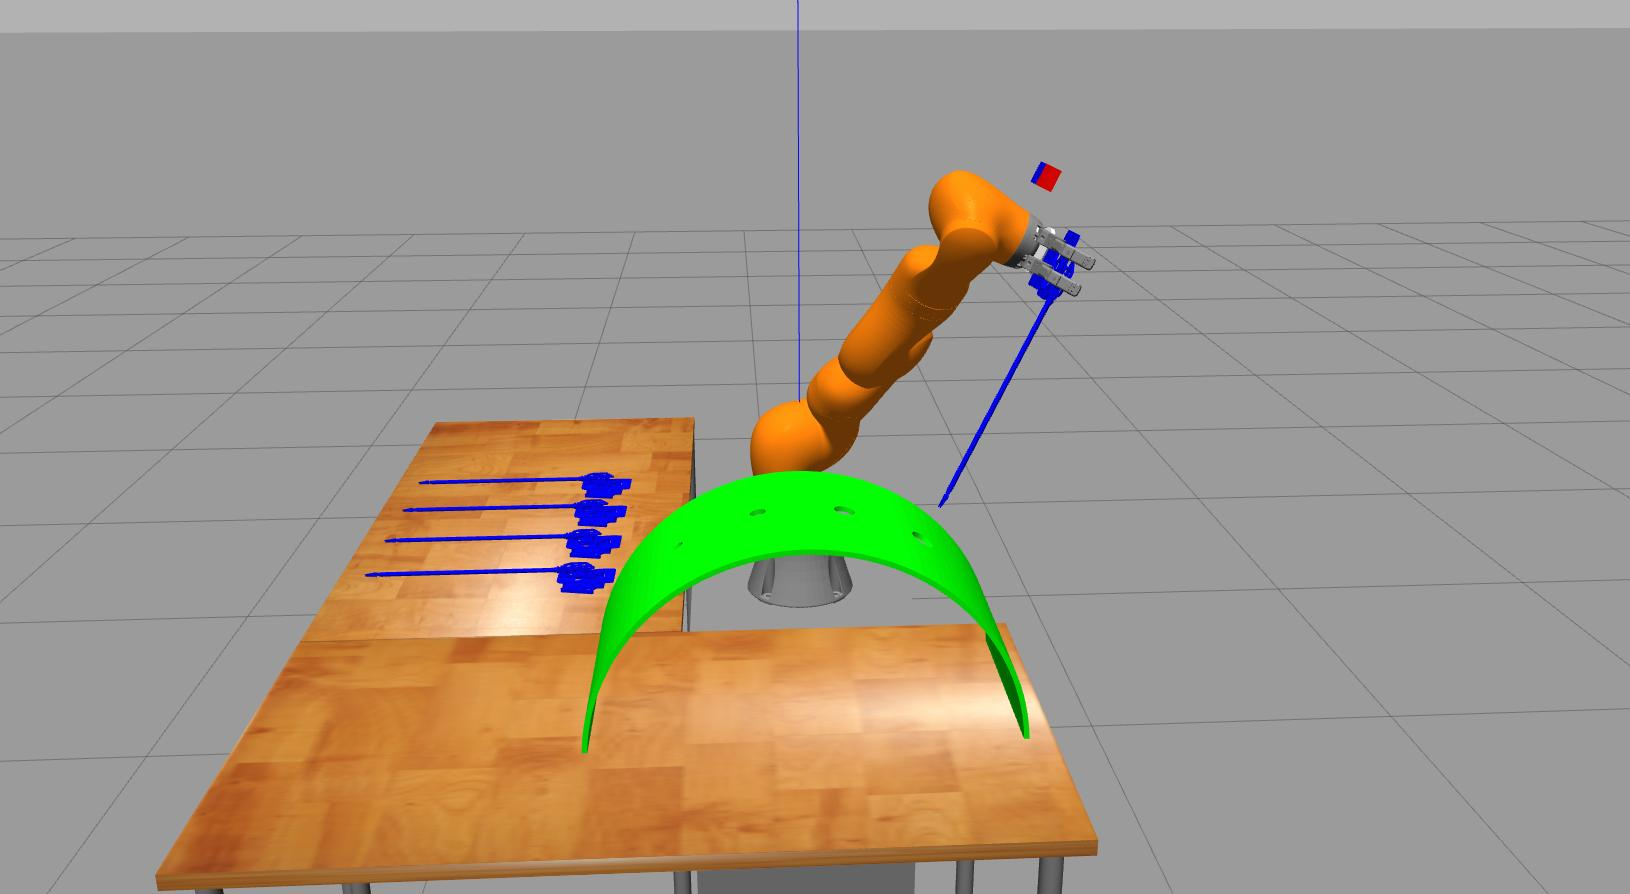
\includegraphics[width=0.3\textwidth]{images/robot_planner2b/robot_planner2b_1}
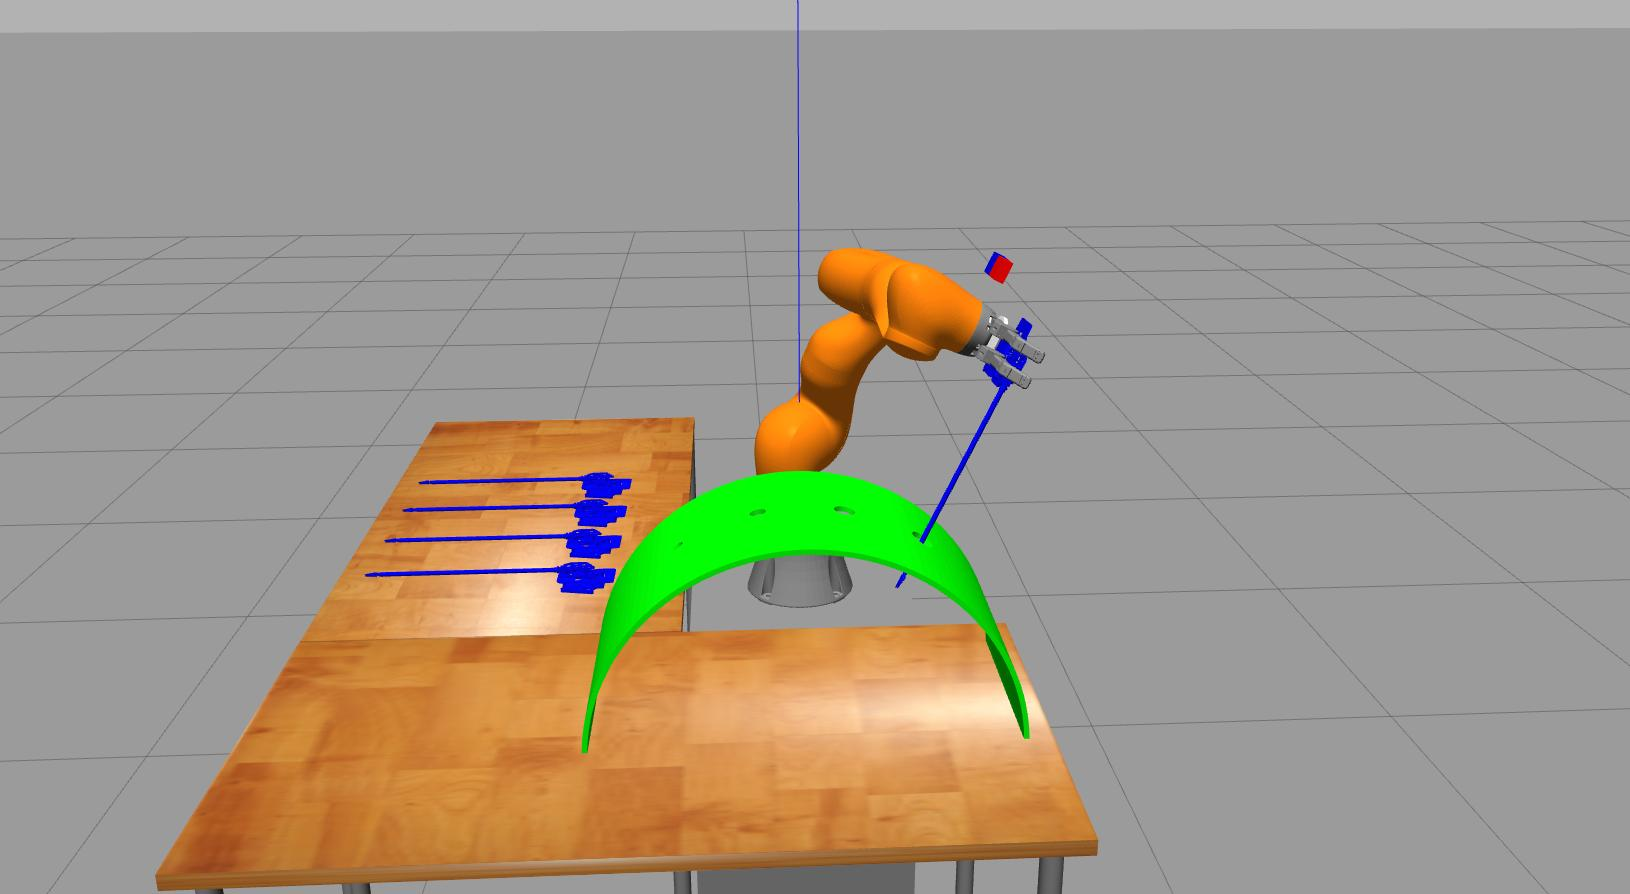
\includegraphics[width=0.3\textwidth]{images/robot_planner2b/robot_planner2b_2}
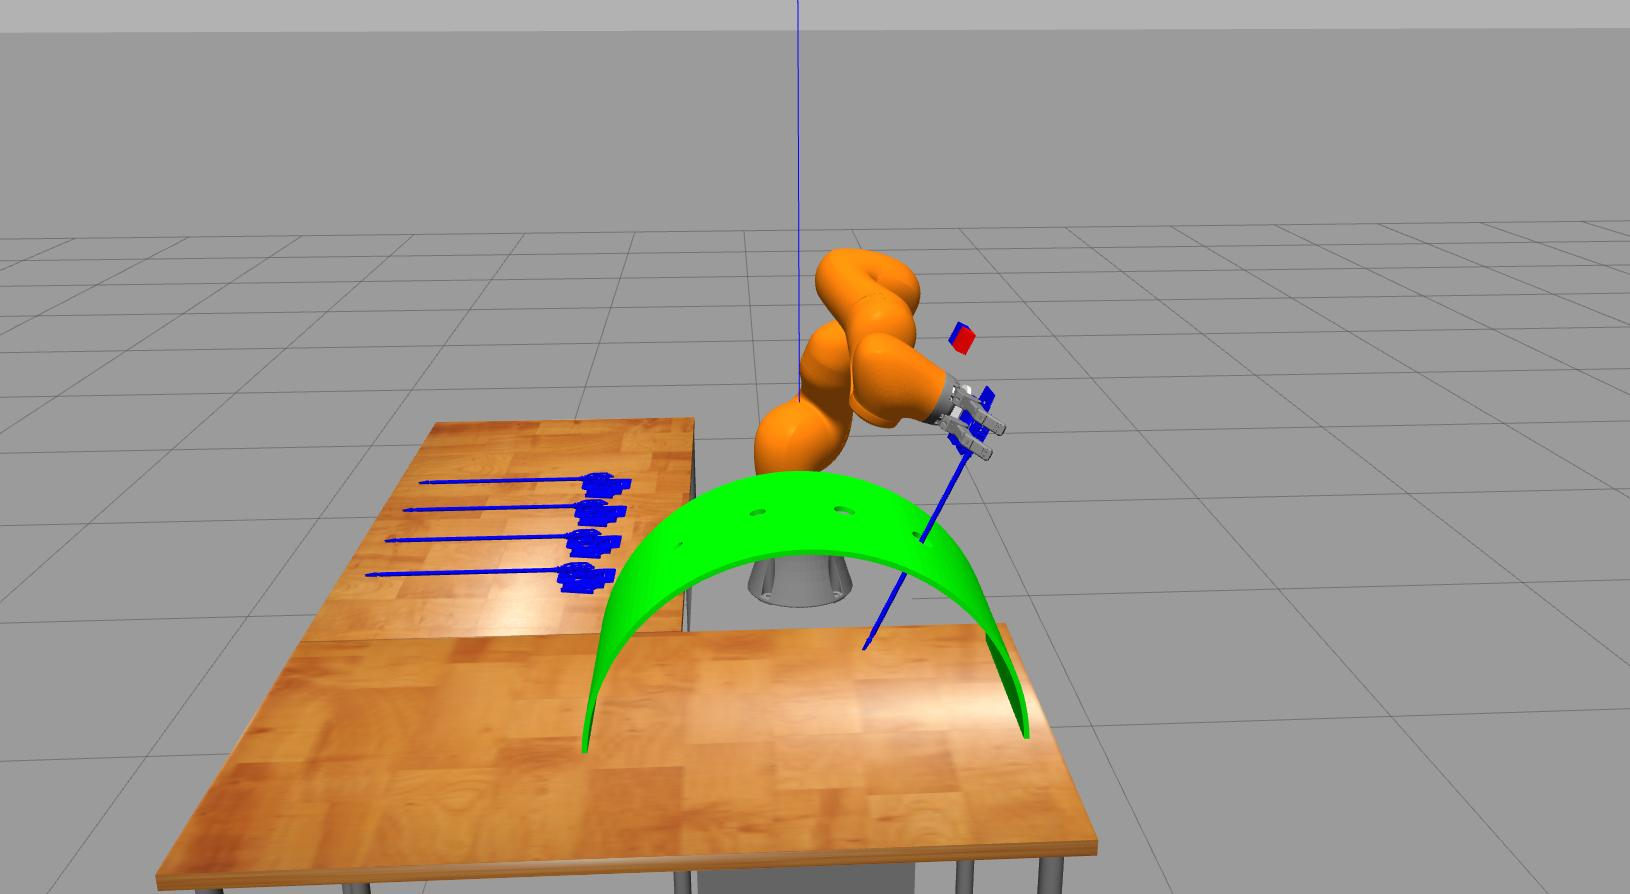
\includegraphics[width=0.3\textwidth]{images/robot_planner2b/robot_planner2b_3}\\
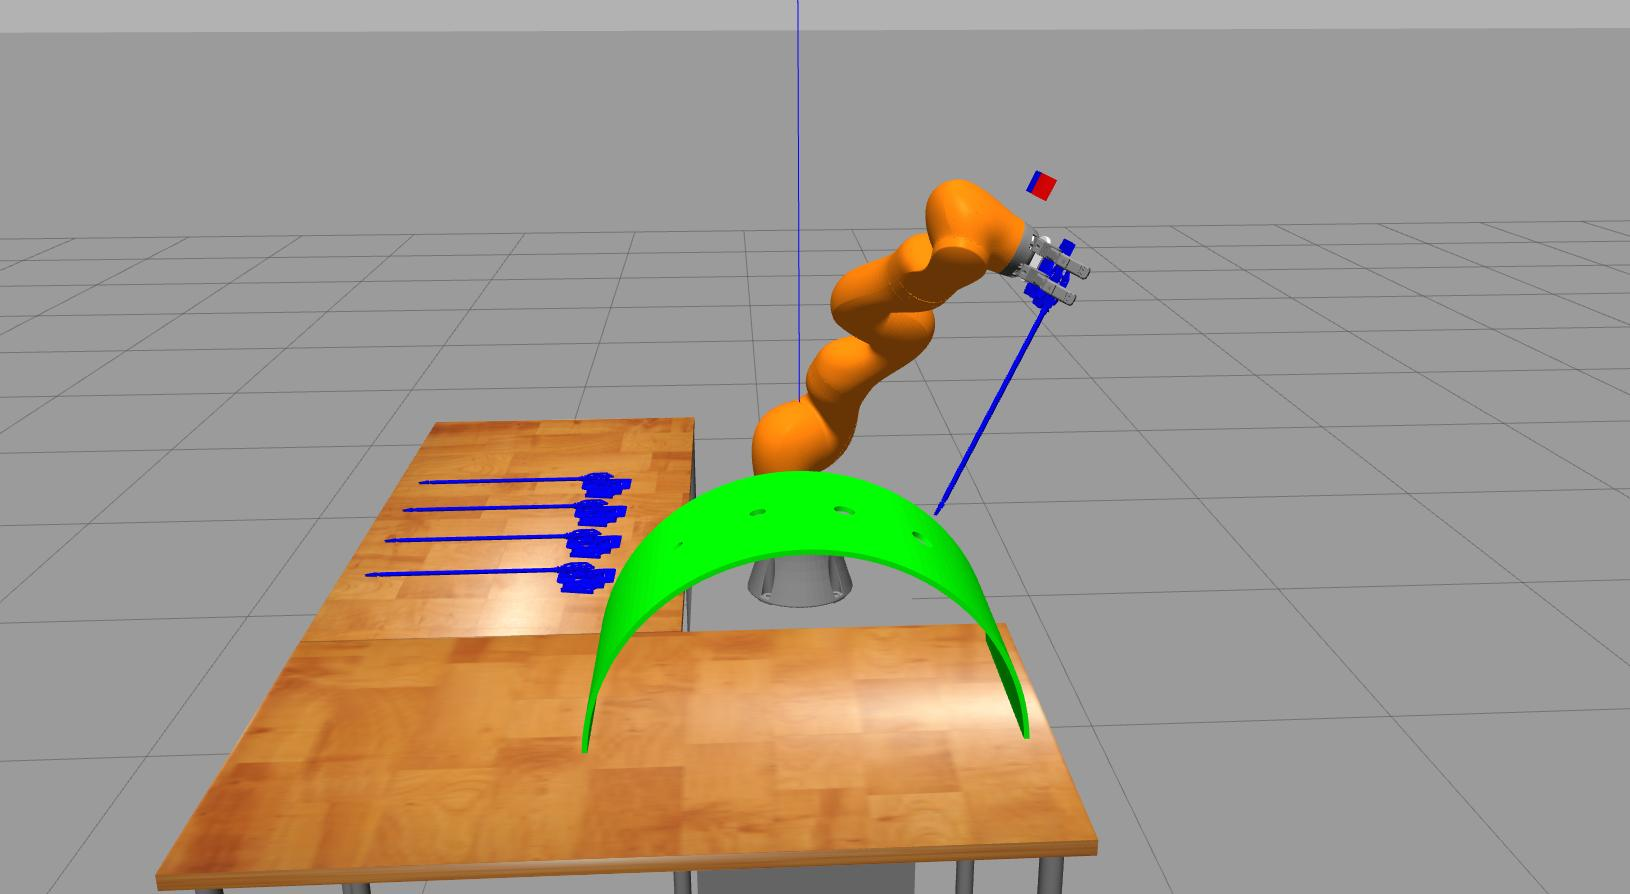
\includegraphics[width=0.3\textwidth]{images/robot_planner2b/robot_planner2b_4}
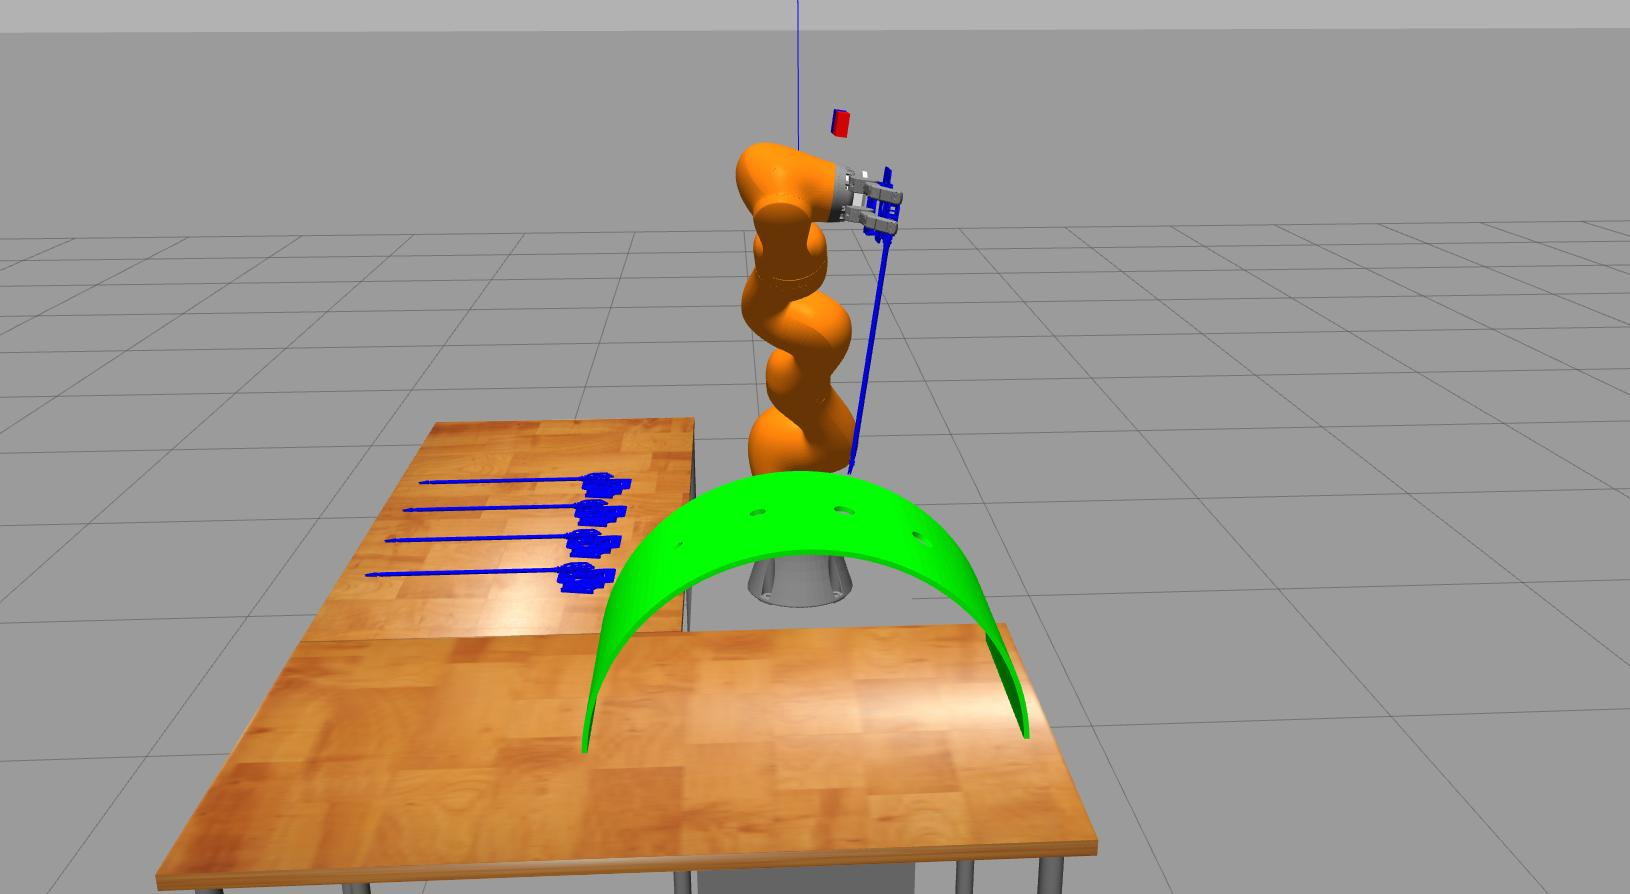
\includegraphics[width=0.3\textwidth]{images/robot_planner2b/robot_planner2b_5}
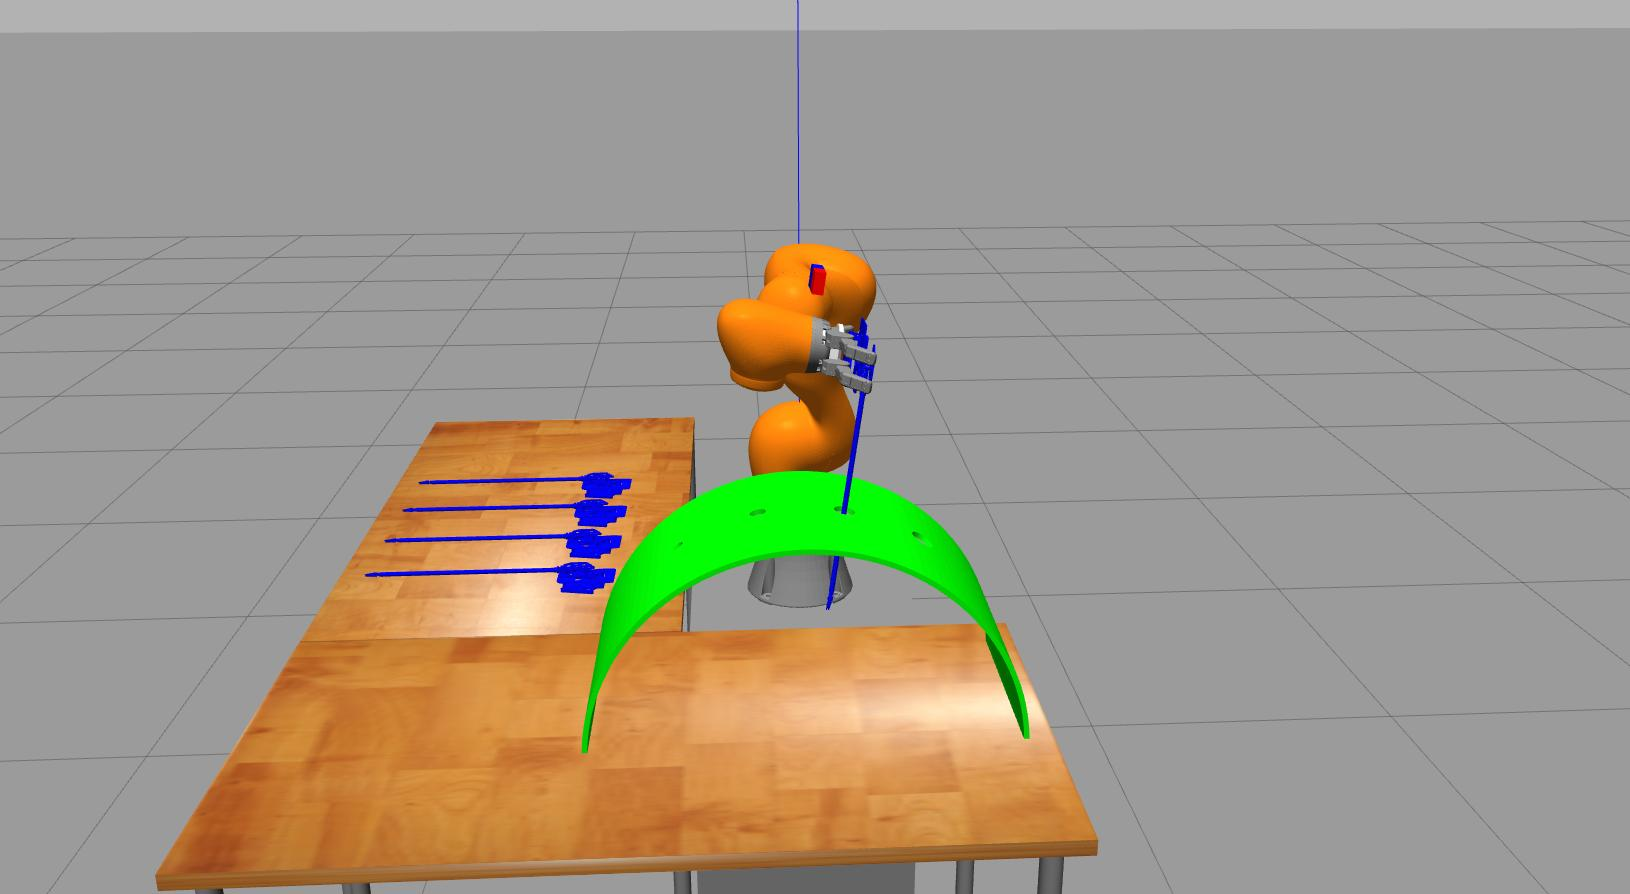
\includegraphics[width=0.3\textwidth]{images/robot_planner2b/robot_planner2b_6}\\
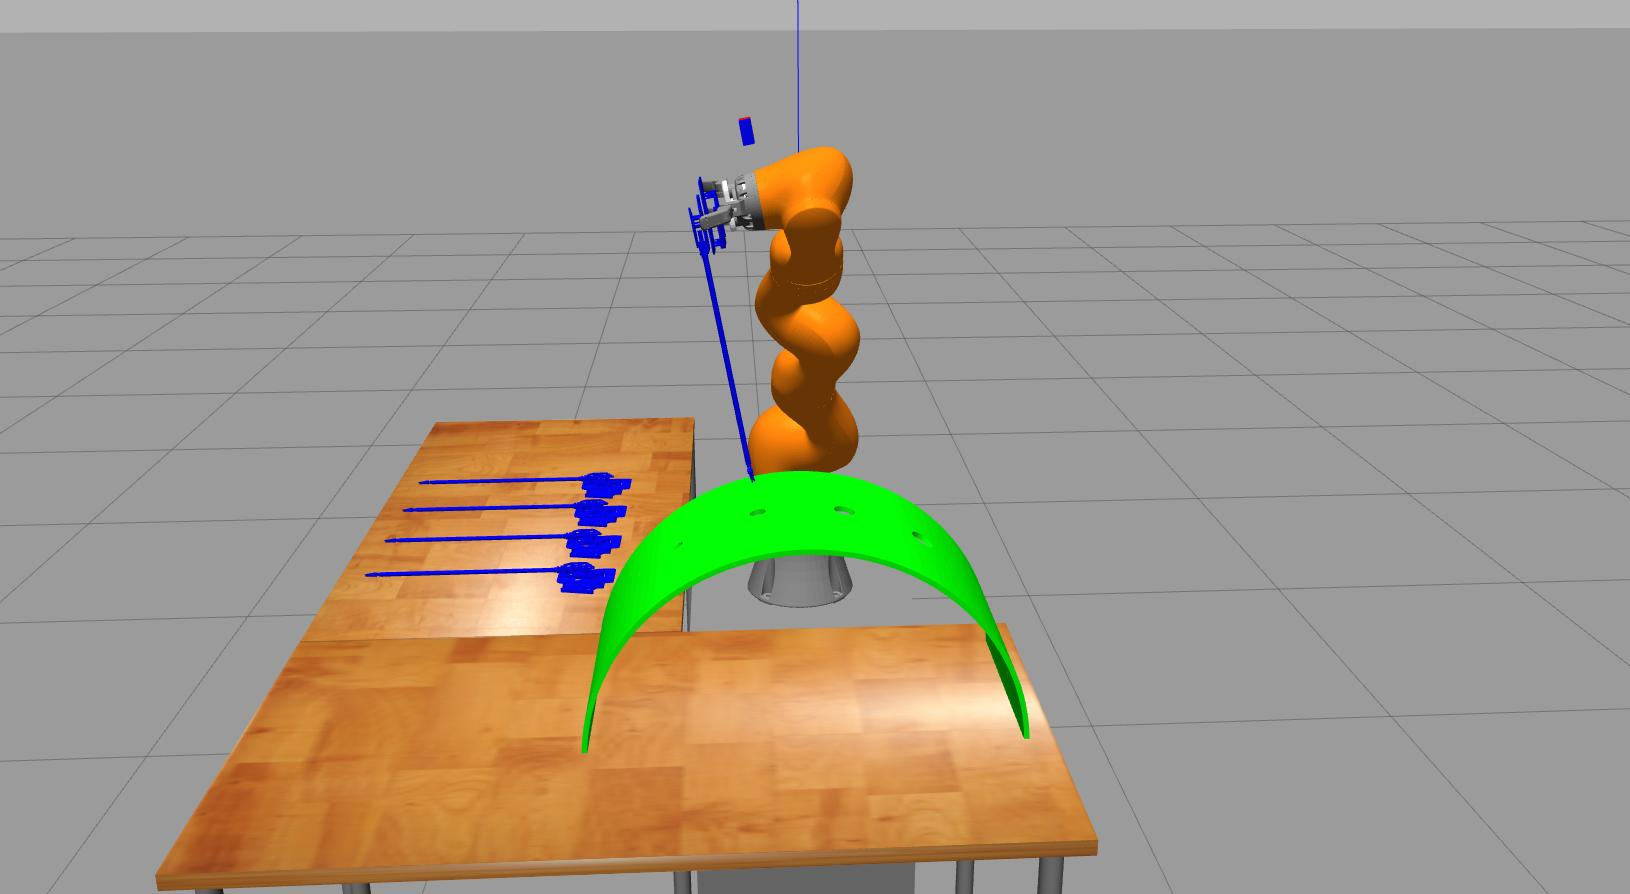
\includegraphics[width=0.3\textwidth]{images/robot_planner2b/robot_planner2b_7}
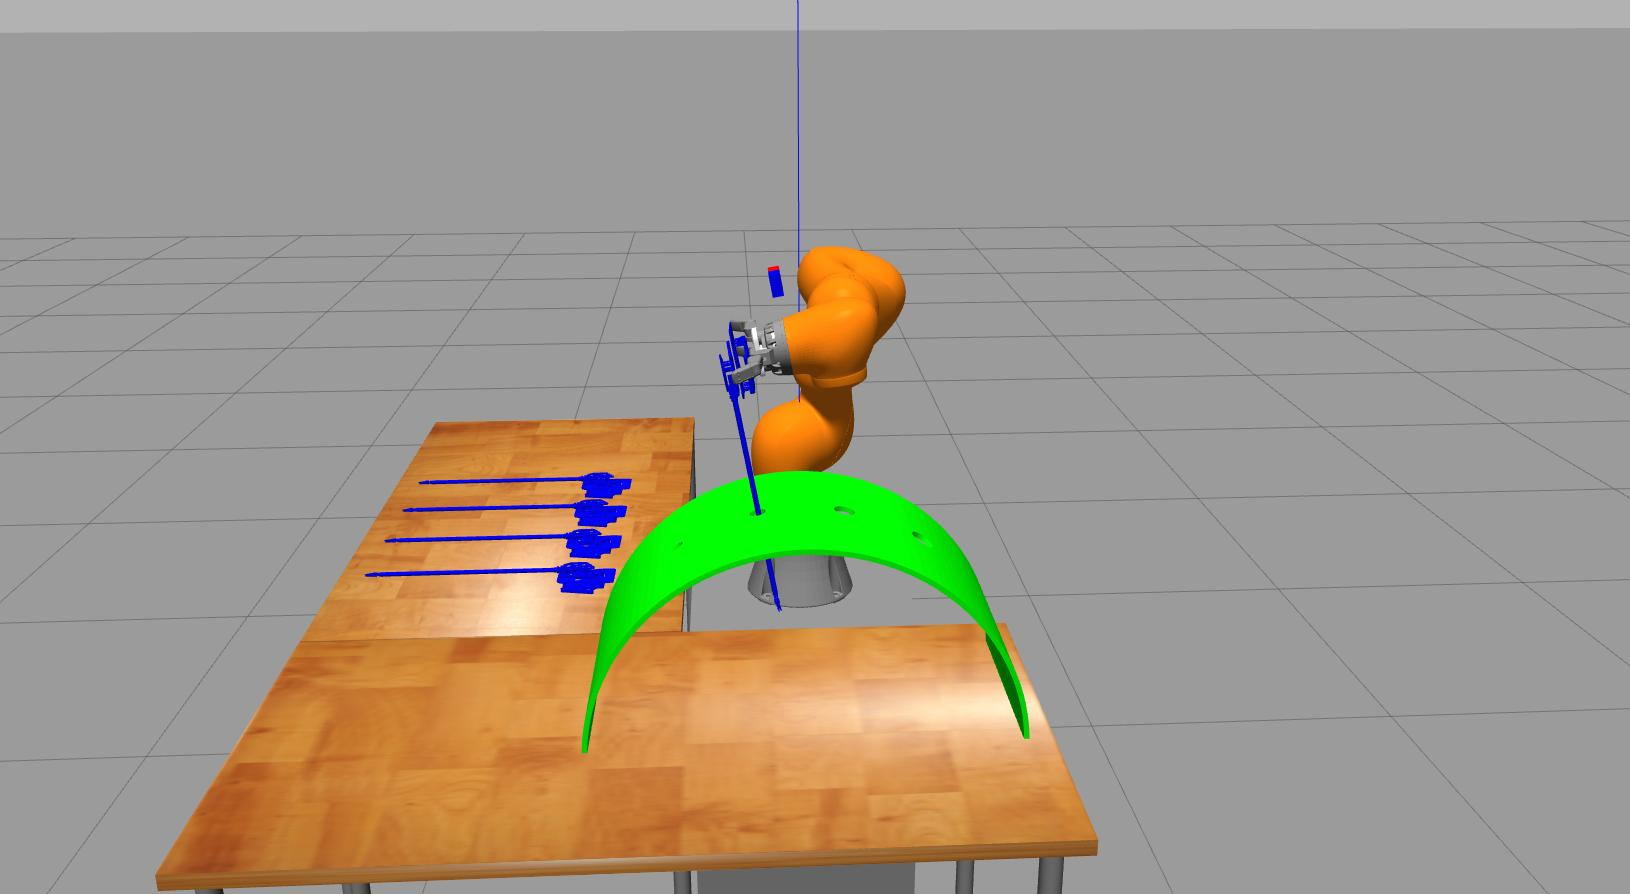
\includegraphics[width=0.3\textwidth]{images/robot_planner2b/robot_planner2b_8}
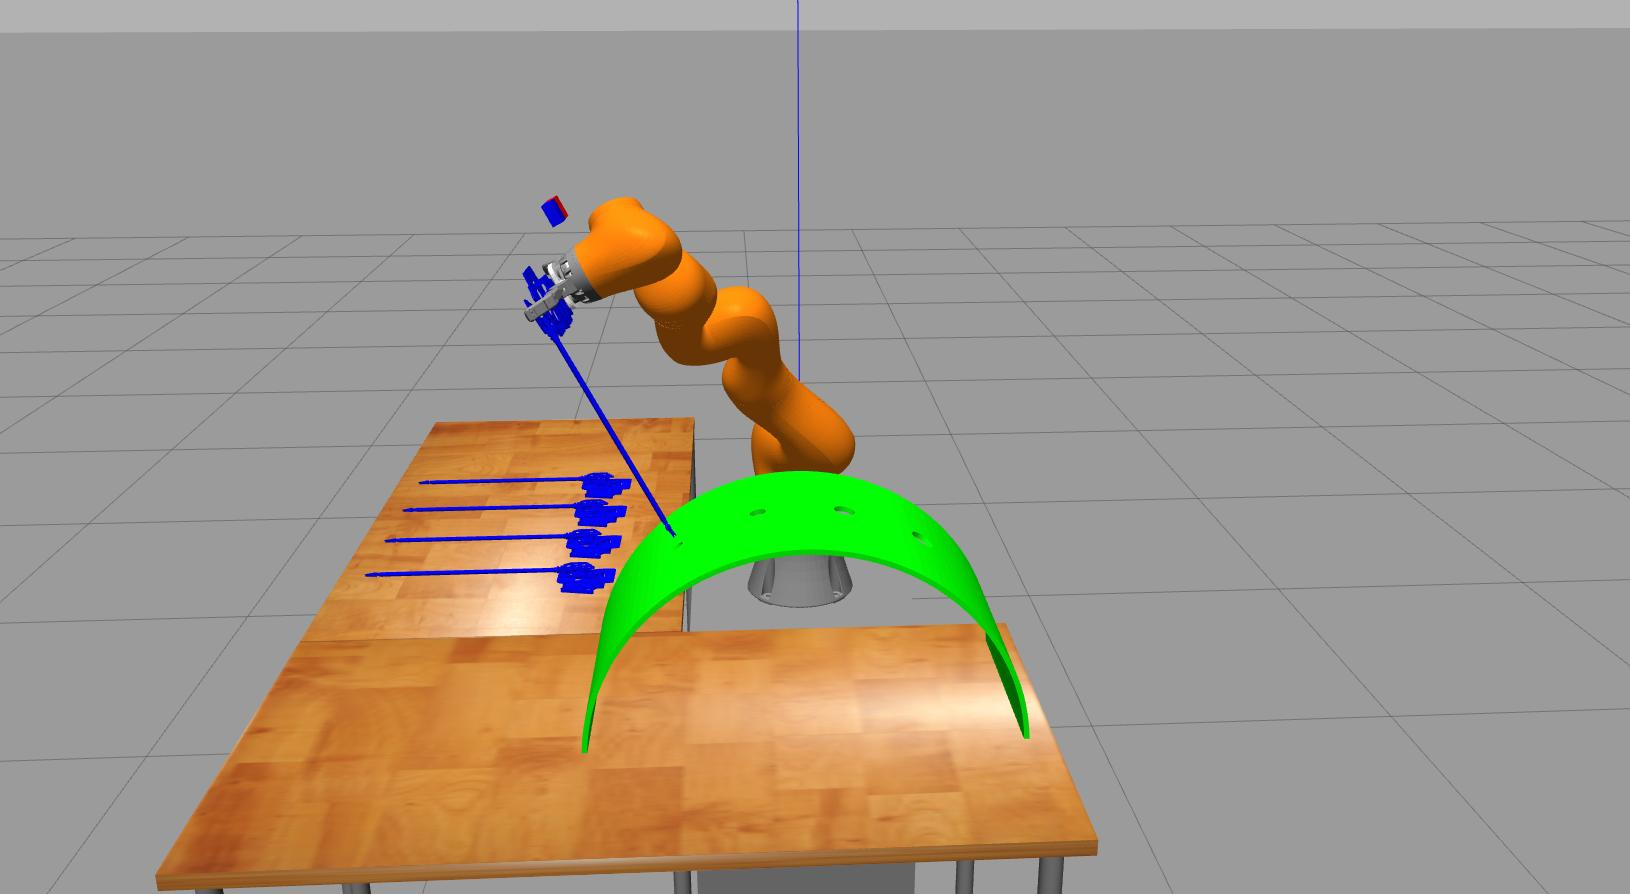
\includegraphics[width=0.3\textwidth]{images/robot_planner2b/robot_planner2b_9}\\
\caption{Experiment 2b:}
\end{figure}
\end{center}

Due to the probabilistic nature of the motion planner (in these experiments the OMPL library is used with the RRTConnect path planning algorithm), the solutions 
to the path planning problem are not always the same and thus it is possible that the robot arm reaches a pose which is close to a singularity
\begin{center}
\begin{figure}[H]
\centering
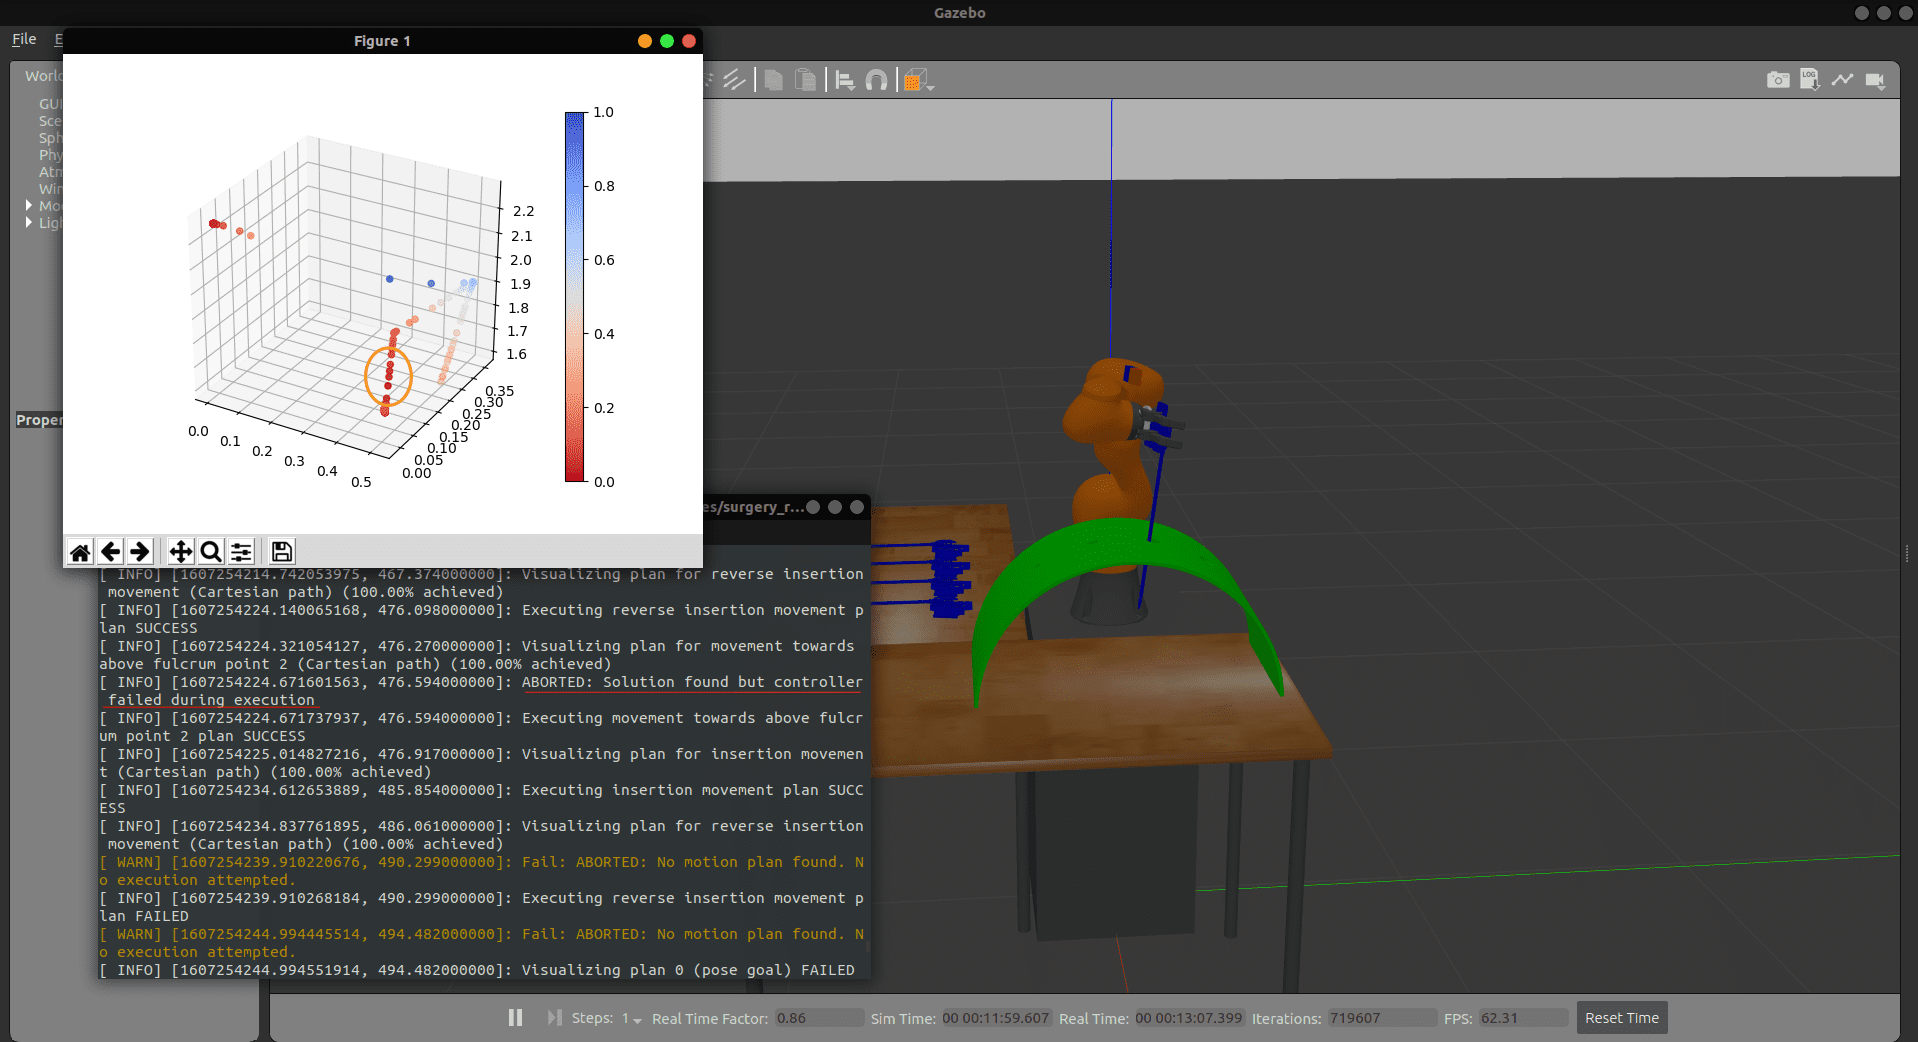
\includegraphics[width=0.9\textwidth]{images/robot_planner2b/singularity_failure.png}
\caption{Experiment 2b: Singularity failure}
\end{figure}
\end{center}

\subsection{Robot Planner 3}

The goal of this third experiment is to design and test only some pivot trajectories. The pivot motions follow the equations described in 
\ref{subsection:pivot-motions}. The trajectories that were designed and tested in this experiments are the following:
\begin{itemize}
\item Circular
\item Arc
\item Line segment
\end{itemize}

\subsubsection{Circular and Circular arc trajectories in task space}

\subsubsection{Line segment trajectories in task space}

\subsubsection{Cubic Spline trajectories in task space}

\subsubsection{B-Spline trajectories in task space}

\subsubsection{Polynomial trajectories in joint space}

\subsubsection{Trajectories in joint space with trapezoidal velocity profile}

\subsubsection{Trajectories in joint space with s-curve velocity profile}

\subsection{Robot Planner 4}

In this experiment we plan a simple pick-and-place path for a cube. The robotic arm first visits the left table and starts from the pre-grasp posture and then 
slowly approaches the cube until the grasp posture. When the gripper has reached the grasp posture, it closes the fingers to grasp the object and then retreats 
to the post-grasp posture. After that the robotic arm visits the right table to execute the place steps which are similar to the pick steps. The images below 
show some frames from the experiment with the first three to show the pick steps in the simulation environment and then other three images show the place steps 
in the visualization program.

\begin{center}
\begin{figure}[H]
\centering
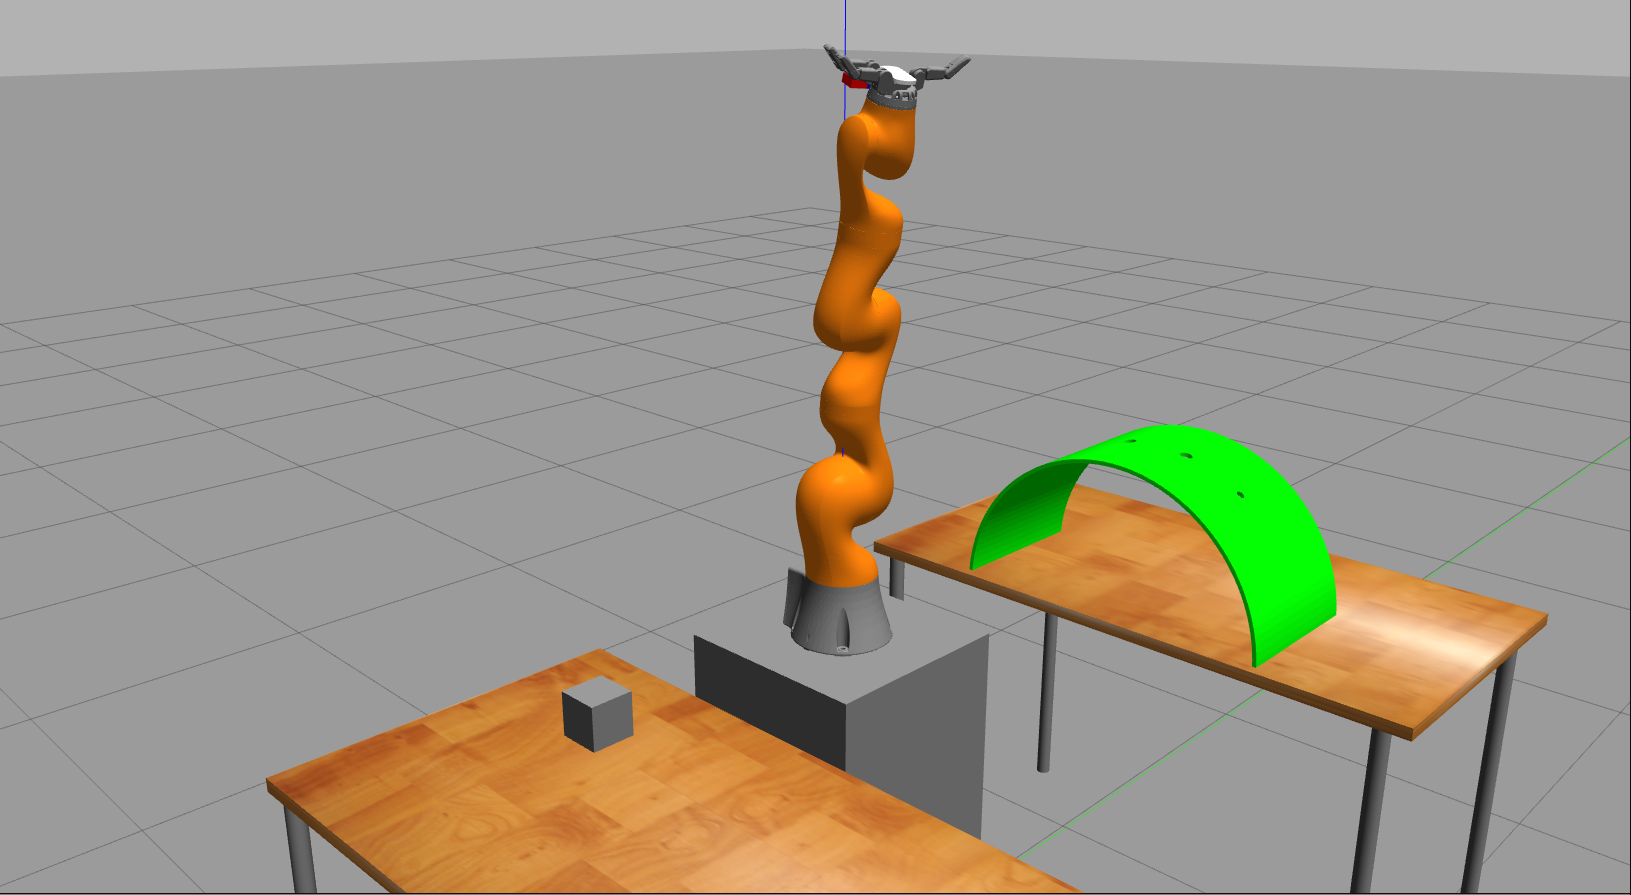
\includegraphics[width=0.3\textwidth]{images/robot_planner4/robot_planner4_1}
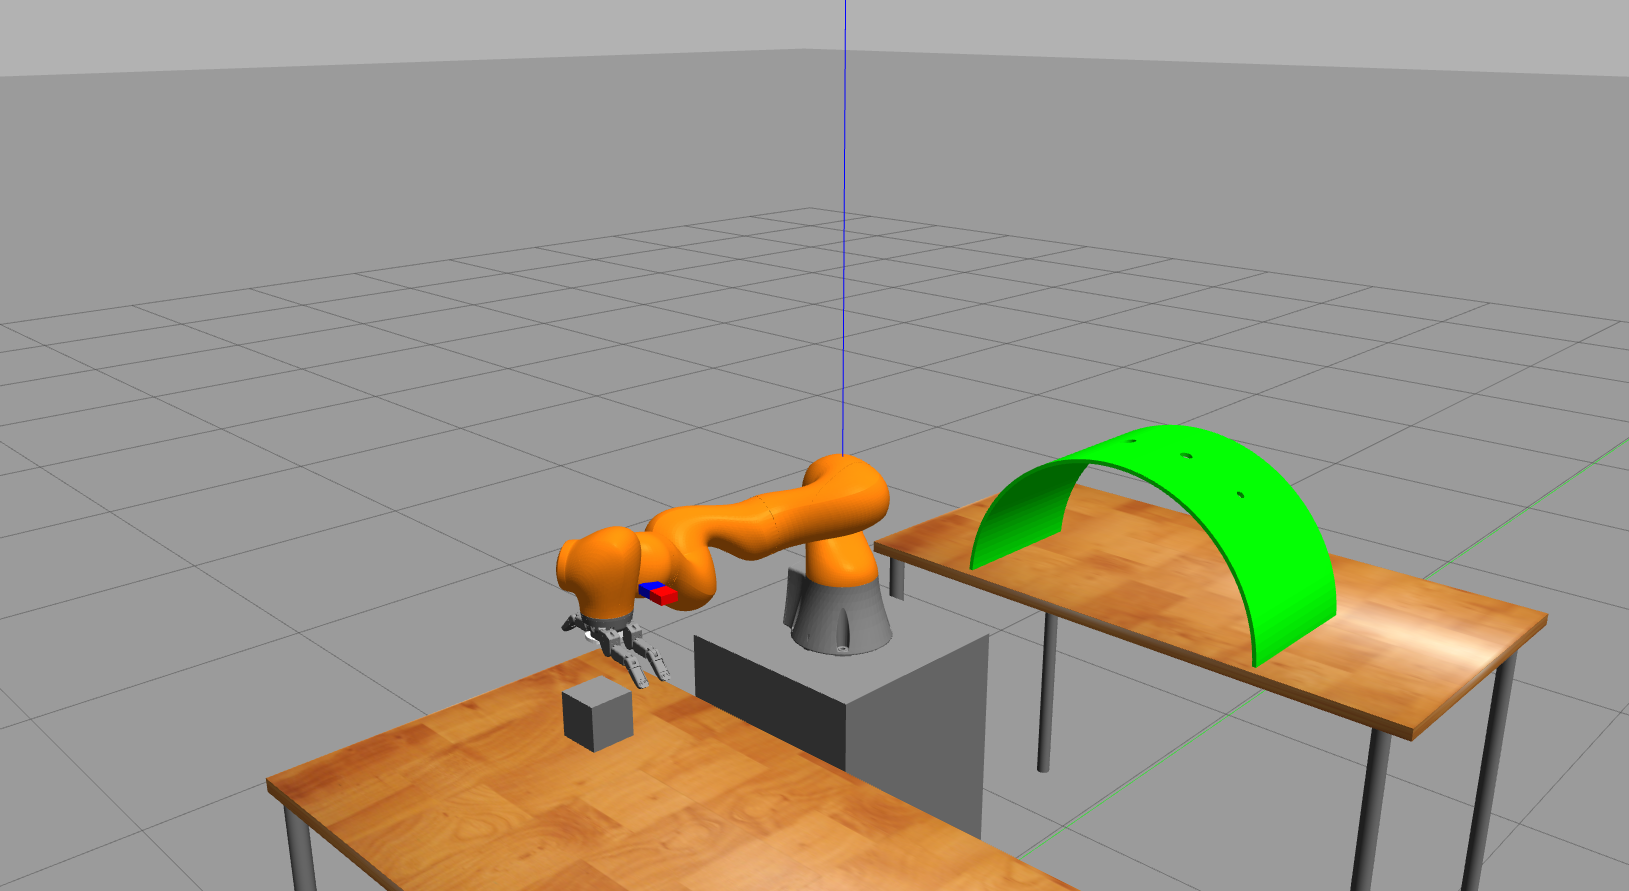
\includegraphics[width=0.3\textwidth]{images/robot_planner4/robot_planner4_3}
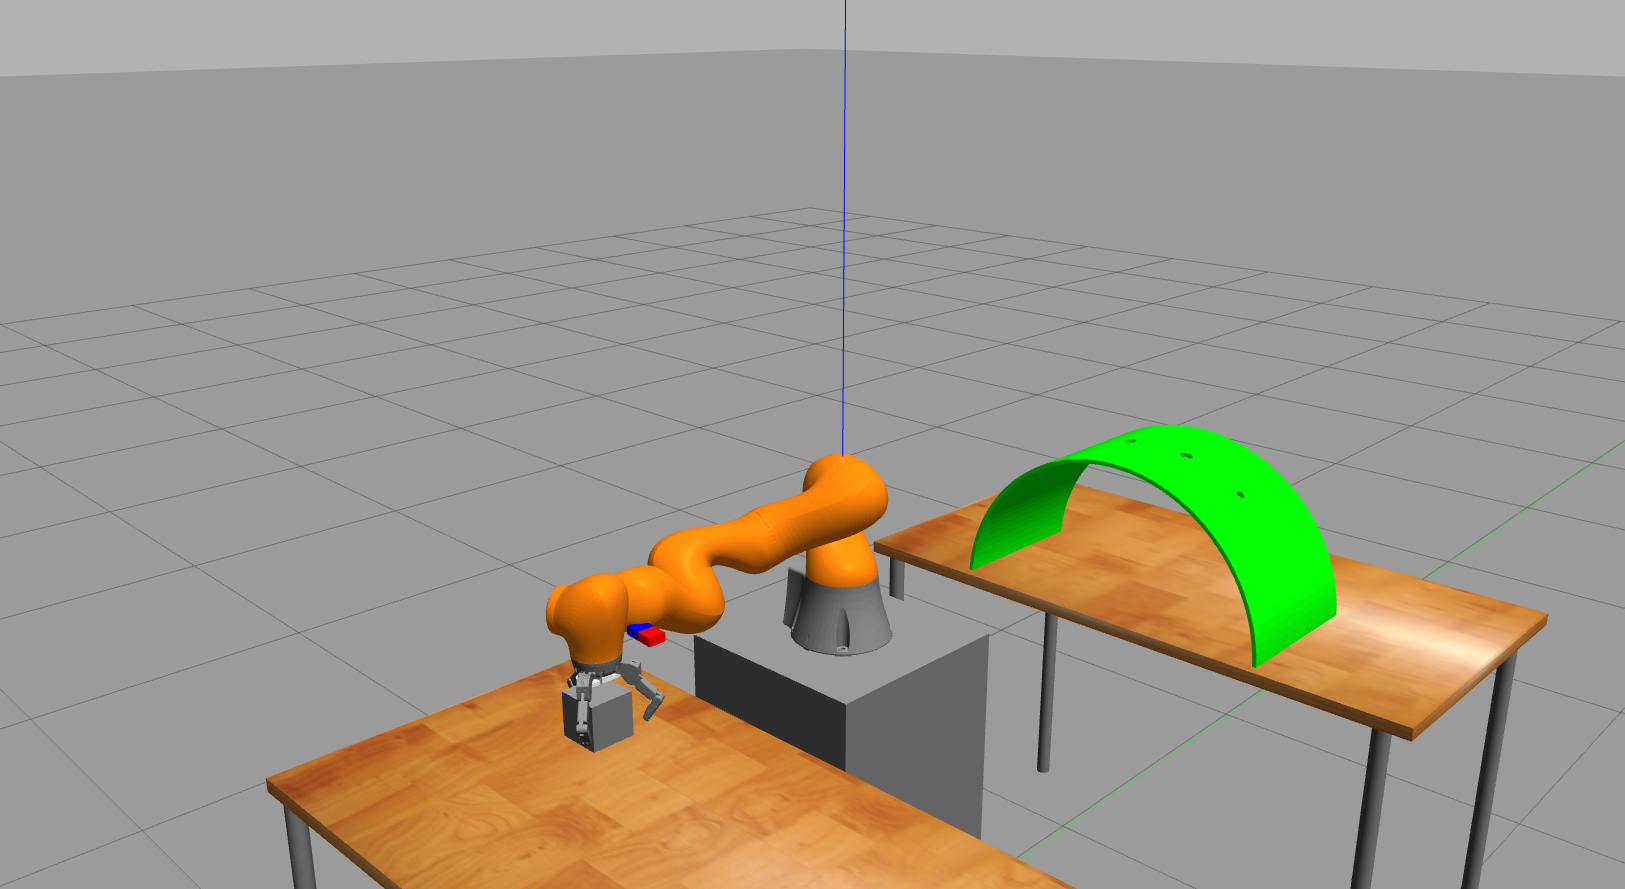
\includegraphics[width=0.3\textwidth]{images/robot_planner4/robot_planner4_5}\\
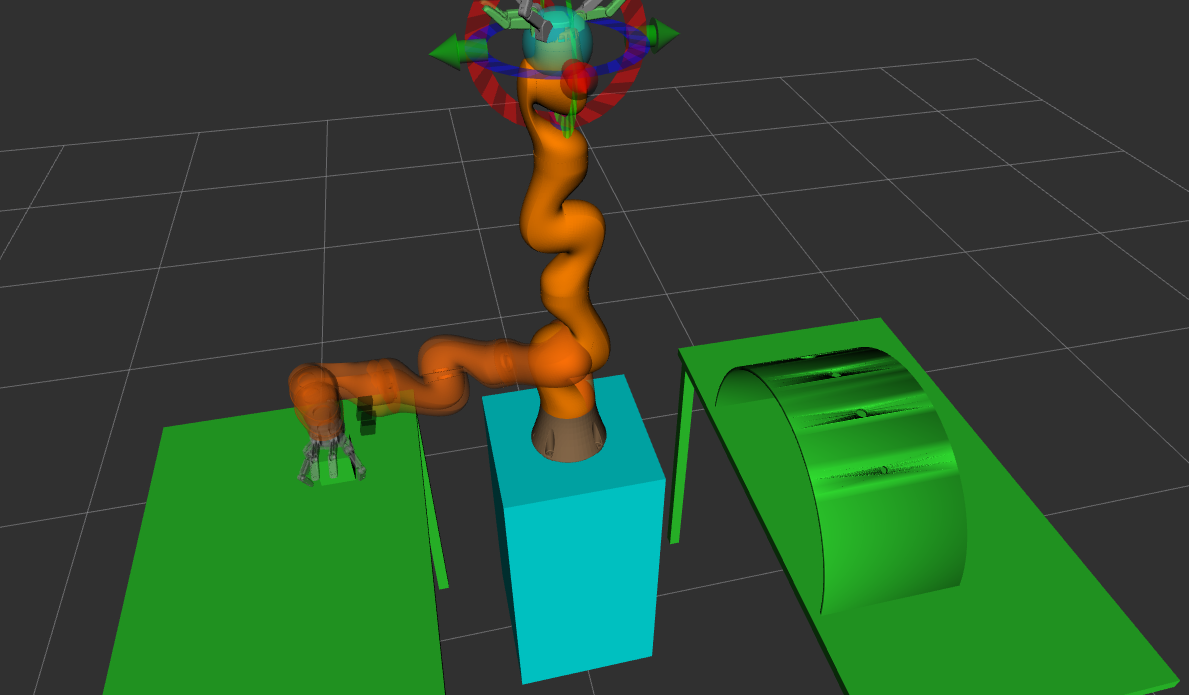
\includegraphics[width=0.3\textwidth]{images/robot_planner4/robot_planner4_6}
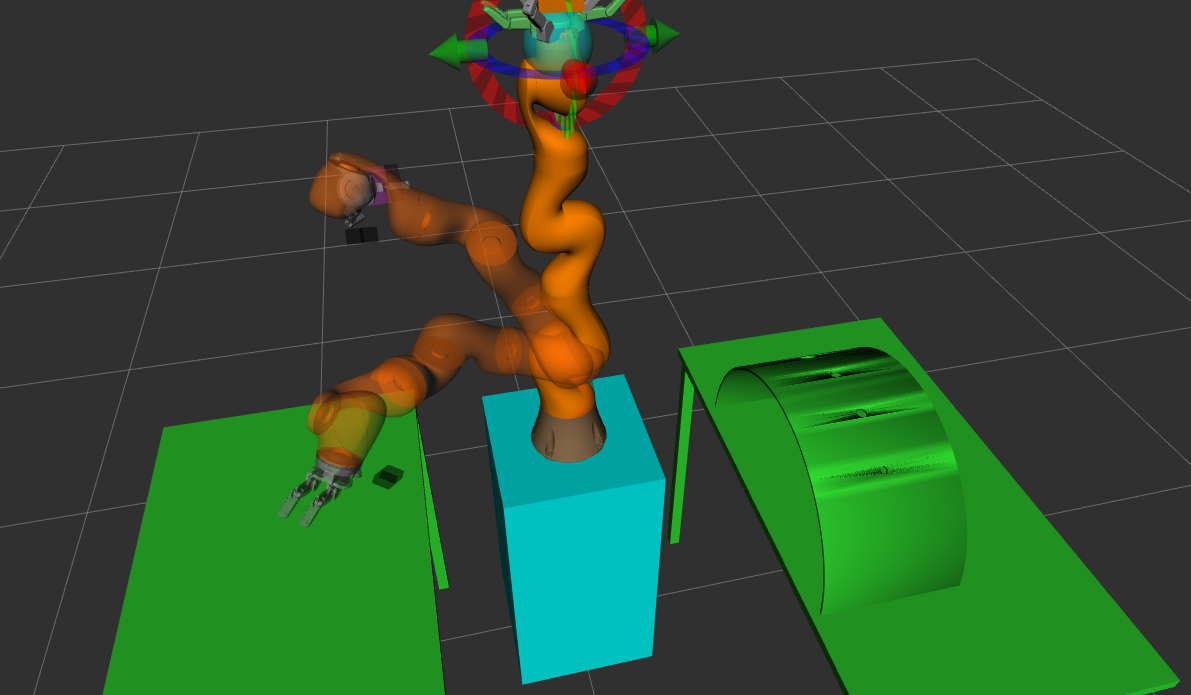
\includegraphics[width=0.3\textwidth]{images/robot_planner4/robot_planner4_8}
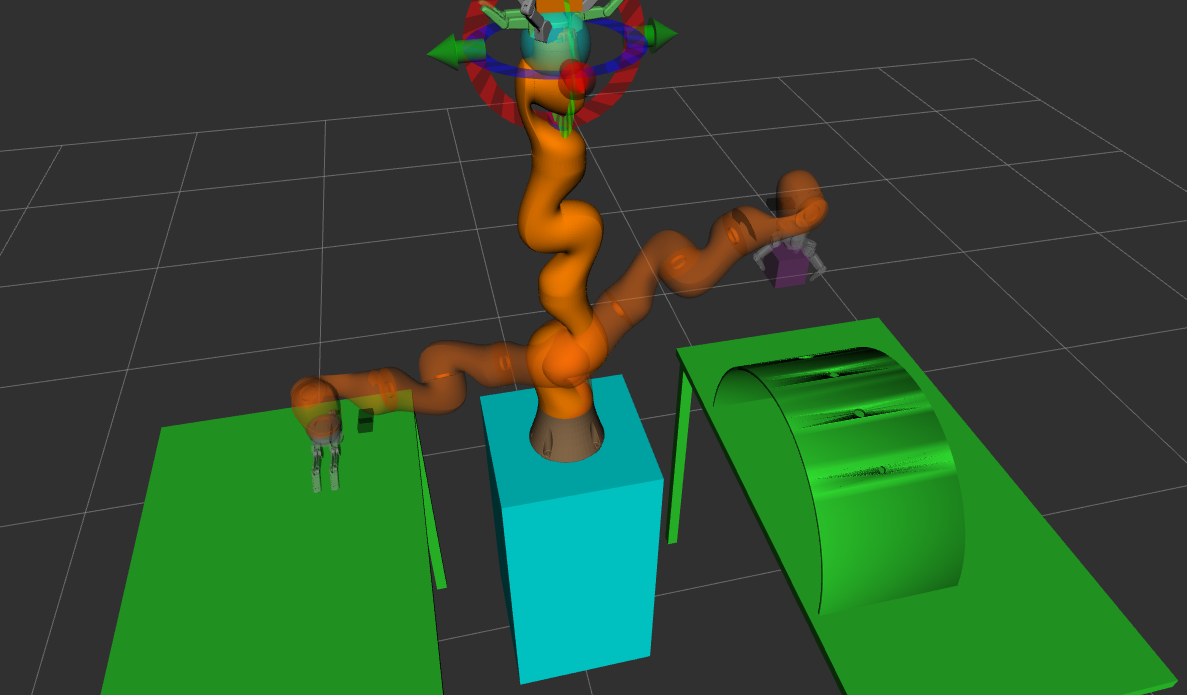
\includegraphics[width=0.3\textwidth]{images/robot_planner4/robot_planner4_10}\\
\caption{Experiment 4: Simple pick-and-place experiment of a cube}
\end{figure}
\end{center}

% Robot Planner 4 with RRTConnect
\begin{table}[H]
\centering
\scalebox{0.8}{
\begin{tabular}{|p{2cm}|c|p{2cm}|p{2cm}|p{2cm}|c|p{2cm}|p{2cm}|p{2cm}|}
\hline
                          & \multicolumn{8}{c}{\textbf{RRTConnect}}                                                                                                 \vline \\
\hline
Robot Planner 4           & \multicolumn{4}{c}{\textbf{Pick Pipeline}}                     \vline & \multicolumn{4}{c}{\textbf{Place Pipeline}}                     \vline \\
\hline
Experiment                & Status & Solution Time & Path Simplification Time & Planning Attempts & Status & Solution Time & Path Simplification Time & Planning Attempts  \\
\hline
1                         & 1      & 0.026189      & 0.065173                 & 1                 & 1      & 0.014644      & 0.020947                 & 1                  \\
2                         &        &               &                          &                   &        &               &                          &                    \\
3                         &        &               &                          &                   &        &               &                          &                    \\
4                         &        &               &                          &                   &        &               &                          &                    \\
5                         &        &               &                          &                   &        &               &                          &                    \\
\hline
\textbf{Average}          &        &               &                          &                   &        &               &                          &                    \\
\hline
\end{tabular}
}
\end{table}

% Robot Planner 4 with RRT*
\begin{table}[H]
\centering
\scalebox{0.8}{
\begin{tabular}{|p{2cm}|c|p{2cm}|p{2cm}|p{2cm}|c|p{2cm}|p{2cm}|p{2cm}|}
\hline
                          & \multicolumn{8}{c}{\textbf{RRT*}}                                                                                                 \vline \\
\hline
Robot Planner 4           & \multicolumn{4}{c}{\textbf{Pick Pipeline}}                     \vline & \multicolumn{4}{c}{\textbf{Place Pipeline}}                     \vline \\
\hline
Experiment                & Status & Solution Time & Path Simplification Time & Planning Attempts & Status & Solution Time & Path Simplification Time & Planning Attempts  \\
\hline
1                         &        &               &                          &                   &        &               &                          &                    \\
2                         &        &               &                          &                   &        &               &                          &                    \\
3                         &        &               &                          &                   &        &               &                          &                    \\
4                         &        &               &                          &                   &        &               &                          &                    \\
5                         &        &               &                          &                   &        &               &                          &                    \\
\hline
\textbf{Average}          &        &               &                          &                   &        &               &                          &                    \\
\hline
\end{tabular}
}
\end{table}

% Robot Planner 4 with PRM*
\begin{table}[H]
\centering
\scalebox{0.8}{
\begin{tabular}{|p{2cm}|c|p{2cm}|p{2cm}|p{2cm}|c|p{2cm}|p{2cm}|p{2cm}|}
\hline
                          & \multicolumn{8}{c}{\textbf{PRM*}}                                                                                                 \vline \\
\hline
Robot Planner 4           & \multicolumn{4}{c}{\textbf{Pick Pipeline}}                     \vline & \multicolumn{4}{c}{\textbf{Place Pipeline}}                     \vline \\
\hline
Experiment                & Status & Solution Time & Path Simplification Time & Planning Attempts & Status & Solution Time & Path Simplification Time & Planning Attempts  \\
\hline
1                         &        &               &                          &                   &        &               &                          &                    \\
2                         &        &               &                          &                   &        &               &                          &                    \\
3                         &        &               &                          &                   &        &               &                          &                    \\
4                         &        &               &                          &                   &        &               &                          &                    \\
5                         &        &               &                          &                   &        &               &                          &                    \\
\hline
\textbf{Average}          &        &               &                          &                   &        &               &                          &                    \\
\hline
\end{tabular}
}
\end{table}


\subsection{Robot Planner 5}

The goal of this fifth experiment is to control the KUKA robot using the camera via the visual servoing technique. In the first part of the experiment the 
robotic arm goes to an initial known position (e.g. the corner of the table) and then moves around until it detects a surgical tool. When that happens, the 
image-based visual servoing will send commands to the robot so that the detected tool is at the center of the video frame and with the same orientation 
as the video frame. At the second part of the experiment, the robot follows a similar algorithm. It starts with a known position, like the corner of the second 
table, then moves around until the mounting dock starts to appear inside the frame. When that happens, the image-based visual servoing will send commands to the 
robot so that the center of the trocar or the fulcrum reference frame is at the center and with the same orientation as the video frame. Similar results can be 
achieved by using position-based visual servoing, but that was not chosen at this implementation for simplicity and less operations. Position-based servoing 
requires more calculations because it is required to get the camera's transformation, express it with respect to the end-effector and then calculate the 
end-effector pose which is then used as an input to a Cartesian Controller.

\begin{center}
\begin{figure}[H]
\centering
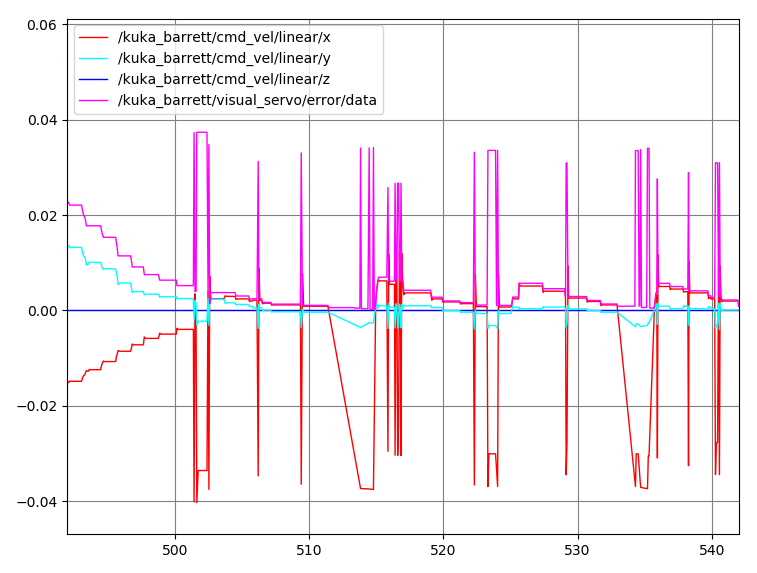
\includegraphics[width=0.45\textwidth]{images/robot_planner5/visual_servo_controller3.png}
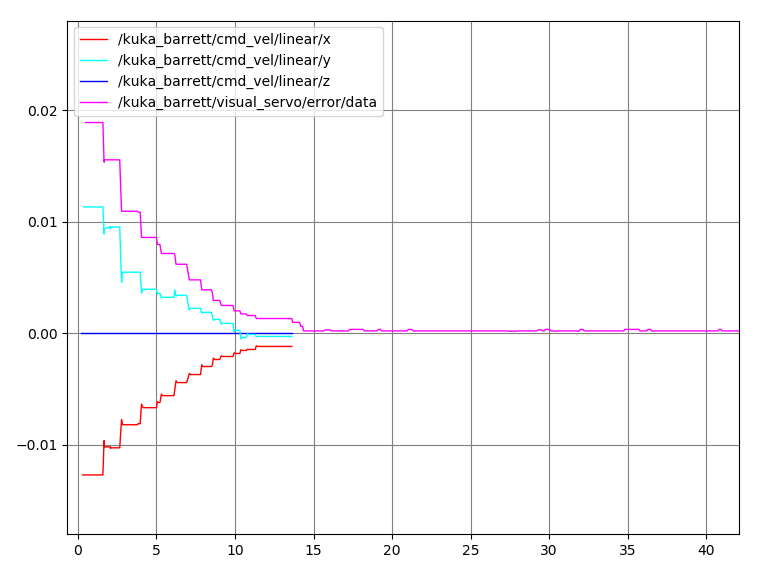
\includegraphics[width=0.45\textwidth]{images/robot_planner5/visual_servo_controller4.png}\\
\caption{Visual servo controller error diagrams. On the left image in the error graphs appear some spikes. These spikes occur from the sudden temporary detection 
of a nearby surgical tool. On the right image, these spikes are filtered out, and only the error graphs of the visual servoing of one tool are shown. The  
controller parameters are $K_p = 0.9, K_d = 0.2$}
\end{figure}
\end{center}

\begin{center}
\begin{figure}[H]
\centering
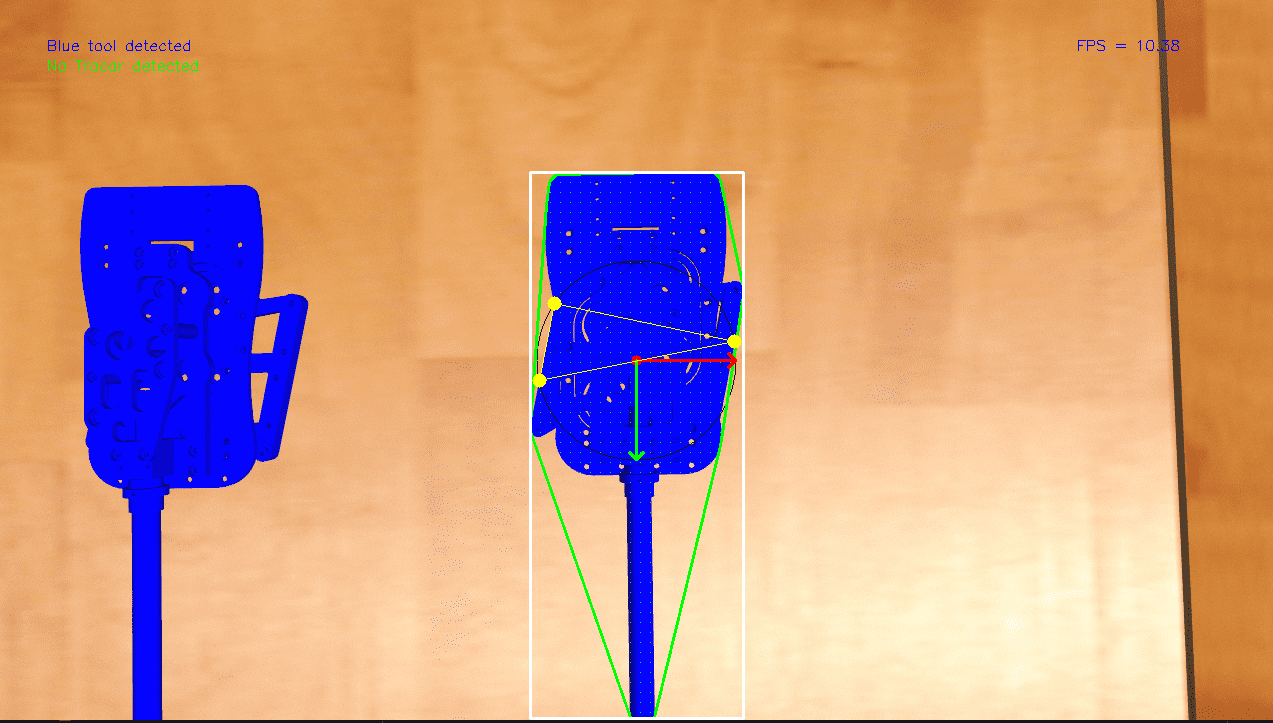
\includegraphics[width=0.6\textwidth]{images/grasp-points-triangle.png}\\
\caption{Image based visual servoing and calculation of grasp points. The yellow points are the grasp points and the thin black circumscribed circle is the growing circle that was used to calculate them.}
\end{figure}
\end{center}

\subsection{Robot Planner 6}

\subsection{Robot Planner 7}